% !TeX root = thesis.tex

\section{Interné lokalizačné systémy}\label{sec:relative}

  Do kategórie interných lokalizačných systémov v~tejto práci zaraďujeme také snímače a~metódy vyhodnotenia údajov z~nich, ktoré na poskytnutie lokalizačnej informácie nevyžadujú žiadnu externú infraštruktúru. Na lokalizáciu využívajú prístup nazývaný \emph{hrubé stanovenie polohy} (angl.\ \emph{dead-reckoning}), v~ktorom je aktuálna poloha odvodená na základe informácií o~predošlých polohách a~aktuálnom smere a~rýchlosti pohybu. V~zásade existujú len dva hlavné spôsoby, ktorými je možné takto odhadnúť polohu. Prvým je zaznamenávanie pohybu prvkov okolitého prostredia, čo využívajú metódy \emph{odometrie}. Alternatívou je zaznamenávanie zmien v~zotrvačnosti robota, na čom sú založené \emph{inerčné systémy}.

  Hlavnou výhodou takýchto spôsobov lokalizácie je, že môžu byť okamžite nasadené v~akomkoľvek neznámom prostredí bez potreby časovo náročnej a~často aj nákladnej inštalácie externých prvkov. Sú dokonca úplne nevyhnutné v~aplikáciách, kde vytvorenie infraštruktúry ani teoreticky neprichádza do úvahy, ako sú napr.\ zasahovanie pri katastrofách a~mimoriadnych situáciách, vojenské či extraterestriálne účely. Ich nevýhodou je však prirodzená náchylnosť na akumuláciu chýb, ktorú je potrebné kompenzovať.
  
  \subsection{Odometria}
    
    Najjednoduchšou implementáciou hrubého stanovenia polohy je odometria. Využíva odometer~--~snímač, ktorý je schopný zaznamenať zmenu kinematiky~--~umiestnený na palube mobilného zariadenia (robota). Na základe uplynutého času, prejdenej dráhy vypočítanej z~odometrie a~orientácie, ktorá musí byť získaná iným spôsobom, je následne odvodený odhad aktuálnej polohy~\cite{duchonSnimaceMobilnejRobotike2012}.

    V~prípade kolesových robotov je obvykle snímaný pohyb kolies, tzv.\ kolesová odometria, a~to najčastejšie pomocou inkrementálnych snímačov polohy~\cite{duchonSnimaceMobilnejRobotike2012}. Princíp odometrie je však možné využiť aj pri spracovaní údajov z~iných snímačov. V~súčasnosti už dobre zaužívanou metódou je vizuálna odometria, ktorá využíva obraz z~kamery, a~pomerne nedávnou oblasťou je spracovanie meraní z~\acrshort{lidar}-u~--~lidarová odometria.

    \subsubsection{Kolesová odometria}

      Kolesová odometria využíva snímanie otáčok kolies, resp.\ motora pomocou optického inkrementálneho snímaču (\acrshort{irc}). Ten je schopný zaznamenávať otáčanie hriadeľa pomocou prerušovania svetelného lúča cez mriežku na rotujúcom disku. Pri jeho otáčaní vznikajú impulzy~--~sínusové alebo pravouhlé~--~ktoré reprezentujú zmenu uhla. Rozlíšenie snímača sa vyjadruje ako počet impulzov (cyklov) na jednu otáčku. Základný typ snímača však nevie určiť smer pohybu, preto sa v~mobilnej robotike používa tzv.\ kvadratúrny inkrementálny snímač. Ten má dva optické kanály posunuté o~90° fázovo, čo umožňuje určiť nielen uhol, ale aj smer otáčania. Navyše, každý impulz možno ďalej interpolovať, čím sa zvyšuje presnosť merania~\cite{duchonSnimaceMobilnejRobotike2012}.

      Výhodou \acrshort{irc} je ich jednoduchosť, nízka cena a~vysoká presnosť v~rámci vnútornej štruktúry robota~--~chyby priamo v~snímači sú spravidla zanedbateľné v~porovnaní s~chybami v~mechanickom prenose (napr.\ v~hriadeli). Najväčším problémom \acrshort{irc} je však akumulácia chýb~--~spôsobená napríklad pretáčaním kolies, nepresným priemerom kolies alebo nerovným povrchom. Preto sú odometrické merania pomocou inkrementálnych snímačov síce veľmi presné v~krátkom časovom horizonte, ale dlhodobo sa ich chyba zväčšuje. Na kompenzáciu sa preto bežne používajú korekčné algoritmy, ako je napríklad Kalmanov filter, ktorý kombinuje výstupy z~viacerých senzorov~\cite{duchonSnimaceMobilnejRobotike2012}.

  \subsection{Vizuálna odometria}

    Vizuálna odometria (\acrshort{vo}) je technika odhadu polohy na základe vstupného obrazu z~jednej alebo viacerých kamier. Na rozdiel od kolesovej odometrie, zaznamenáva posunutie obrazu medzi za sebou nasledujúcimi snímkami. Funguje v~reálnom čase, v~porovnaní s~kolesovou odometriou má podstatne vyššiu spoľahlivosť a~je vhodná v~prostrediach bez dostupnosti signálu \acrshort{gps}\@.

    Podľa počtu použitých kamier sa rozlišujú tri typy vizuálnej odometrie~\cite{krombachCombiningFeatureBasedDirect2017}:
    \begin{enumerate}
      \item \emph{Monokulárna}~--~využíva jednu kameru, meria posuny obrazu medzi snímkami a~odhaduje pohyb, jej nevýhodou je faktor neurčitej mierky, ktorý je nutné kompenzovať prídavnými senzormi;
      \item \emph{Stereovízna}~--~kombinuje dve synchronizované kamery, získava hĺbku priamo pomocou stereo triangulácie, čím odstraňuje problém neurčitej mierky;
      \item \emph{Všesmerová}~--~pozostáva z~komplexného systému viacerých mono- alebo stereo-kamier. Poskytuje veľmi široké zorné pole (až do 360°), vďaka čomu je rotačne invariantná. Vyžaduje však presnú kalibráciu a~synchronizáciu medzi kamerami a~je nákladnejšia~\cite{aqelReviewVisualOdometry2016}.
    \end{enumerate}

    \begin{figure}[b!]
      \centering
      \begin{subfigure}[t]{0.48\textwidth}
        \centering
        \vspace*{\fill}
        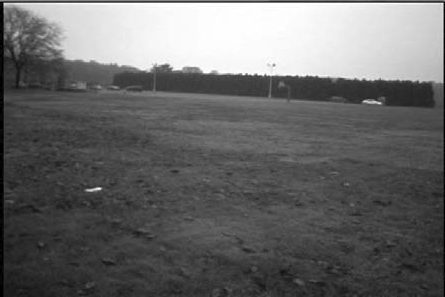
\includegraphics[width=\textwidth]{img/visual_odometry1.png}
        \vspace*{\fill}
        \caption{vstupný obraz}
      \end{subfigure}
      \hfill
      \begin{subfigure}[t]{0.48\textwidth}
        \centering
        \vspace*{\fill}
        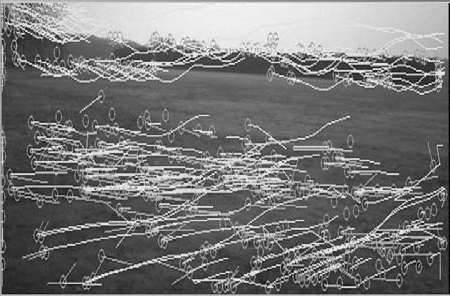
\includegraphics[width=\textwidth]{img/visual_odometry2.png}
        \vspace*{\fill}
        \caption{výstup zo sledovača textúr~--~krúžky reprezentujú aktuálne pozície textúr, čiary sú znázorňujú ich pohyb po obrázku}
      \end{subfigure}
      \caption[Princíp textúrnej vizuálnej odometrie]{Princíp textúrnej vizuálnej odometrie~\cite{nisterVisualOdometry2004}}\label{fig:vo}
    \end{figure}

    Existuje viacero spôsobov určovania pohybu na základe obrazu z~kamier. Medzi dominujúce prístupy \acrshort{vo} patria~\cite{krombachCombiningFeatureBasedDirect2017}:
    \begin{itemize}
      \item \emph{Textúrna}~--~(obr.~\ref{fig:vo}) pracuje s~detekciou a~sledovaním výrazných obrazových prvkov~--~textúr (napr.\ rohy, línie, krivky, \dots). Je presná v~dobre štruktúrovanom prostredí, avšak jej robustnosť klesá pri monotónnych scénach. Na kompenzáciu driftu sa často požíva v~kombinácii s~metódami optimalizácie pozičného grafu.
      \item \emph{Priama}~-~pracuje priamo s~intenzitami všetkých pixelov snímku, bez predchádzajúcej extrakcie, a~to za účelom minimalizácie fotometrickej chyby. Je preto výpočtovo náročnejšia a~pomalšia než textúrna vizuálna odometria. Je tiež citlivejšia na svetelné zmeny.
      \item \emph{Hybridná}~--~využíva kombináciu dvoch predošlých typov na rekonštrukciu trojrozmerného prostredia. V~prvom slede sa použije textúrna \acrshort{vo} na získanie hrubého odhadu polohy, ktorý je neskôr spresnený pomocou priamej \acrshort{vo}.
      \item \emph{vizuálno-inerciálna}~--~kombinuje kameru s~\acrshort{imu}, čo zlepšuje metriku aj stabilitu: \acrshort{imu} poskytuje rýchlo-časové odhady a~pomáha pri rýchlych pohyboch či nízkej textúre. Niektoré takéto systémy dosahujú centimetrovú presnosť a~robustnosť v~náročných prostrediach~\cite{qinVINSMonoRobustVersatile2018}.
    \end{itemize}

    Vďaka efektívnejšiemu výkonu sú v~súčasnosti rozšírenejšie skôr textúrne než priame metódy \acrshort{vo}. Základné problémy, ktoré musí riešiť každý algoritmus textúrnej \acrshort{vo} sú rekonštrukcia pohybu, nelineárna optimalizácia, párovanie textúr, rekonštrukcia hĺbky a~aktualizácia stavu. Ich princíp vysvetlíme v~nasledujúcich častiach podľa~\cite{chienWhenUseWhat2016}.
    
    \subsubsection{Rekonštrukcia pohybu}

      Pre rekonštrukciu pohybu kamery je potrebné získať 3D súradnice bodu na obraze z~kamery. To je možné na základe tzv.\ \emph{dierkového modelu kamery} (angl.\ \emph{pinhole camera model}, viď obr.~\ref{fig:pinhole}). Pre bod v~priestore $\mathbf P = {(x,y,z)}^{\top}$ a~jeho projekciu v~rovine obrazu $\mathbf p = {(u,v)}^{\top}$ je projekčný model definovaný takto:
      \begin{equation}
        \begin{bmatrix}
            \bf p \\ 1
        \end{bmatrix}
        \sim
        \begin{bmatrix}
            f_u & 0 & u_c & 0 \\
            0 & f_v & v_c & 0 \\
            0 & 0 & 1 & 0
        \end{bmatrix}
        \begin{bmatrix}
            \bf P \\ 1
        \end{bmatrix}
        =
        \bf K
        \begin{bmatrix}
            \bf I & \bf 0
        \end{bmatrix}
        \bf P,
      \end{equation}
      kde $\mathbf K$ je tzv.\ \emph{matica kamery}, ktorá obsahuje vnútorné parametre kamery: fokálne vzdialenosti $f_u, f_v$ a~súradnice stredu optickej osi $(u_c,v_c)$.

      \begin{figure}[t!]
        \centering
        \resizebox{0.9\textwidth}{!}{\input{img/pinhole.pdf_tex}}
        \caption[Dierkový model kamery]{Dierkový model kamery~--~projekcia 3D bodu do 2D obrazu kamery (podľa~\cite{CameraCalibration3D})}\label{fig:pinhole}
      \end{figure}
      
      Za predpokladu, že $\mathbf P$ je stacionárny bod v~priestore, jeho projekcia v~nasledujúcej snímke z~kamery sa dá vyjadriť ako
      \begin{equation}
        \begin{bmatrix}
          \bf p' \\ 1
        \end{bmatrix} \sim
        \bf K~
        \begin{bmatrix}
          \bf R & \bf t
        \end{bmatrix}
        \begin{bmatrix}
          \bf P \\ 1
        \end{bmatrix},
        \label{eq:camera-transform}
      \end{equation}
      kde rotačná matica $\mathbf R \in SO(3)$ a~translačný vektor $t \in \mathbb{R}^3$ predstavujú Euklidovskú transformáciu danú pohybom kamery.

      V~kontexte problému odhadu pohybu je transformácia $\begin{bmatrix} \mathbf{R}\ \mathbf{t} \end{bmatrix}$ riešenou neznámou, ktorú je potrebné určiť na základe množiny 3D--2D korešpondencií $(x, y, z) \leftrightarrow (u', v')$. Tento problém je známy ako úloha \emph{perspective-from-n-points} (\acrshort{pnp}). Ak sa na celú projekčnú maticu $\mathbf{P} = \mathbf{K} \begin{bmatrix} \mathbf{R} & \mathbf{t} \end{bmatrix}$ pozeráme ako na problém čiernej skrinky (t.\ j.\ bez znalosti vnútorných závislostí), riešenie je možné získať jednoducho vyriešením homogénneho lineárneho systému. Takýto prístup je známy ako metóda \emph{priamej lineárnej transformácie} (\acrshort{dlt})~\cite{chienWhenUseWhat2016}. Rotácia určená týmto spôsobom však nemusí byť platným prvkom špeciálnej ortogonálnej skupiny $SO(3)$ kvôli nadbytočnej parametrizácii. Preto sa na nájdenie riešenia rovnice~\ref{eq:camera-transform} v~praxi často používa algoritmus \emph{Efficient PnP} (\acrshort{epnp})~\cite{lepetitEPnPAccurateSolution2009}, ktorý ponúka výpočtovo efektívne a~stabilné riešenie úlohy \acrshort{pnp}. Jeho hlavnou výhodou je, že reprezentuje 3D body ako lineárnu kombináciu štyroch kontrolných bodov, čím znižuje počet neznámych a~dosahuje lineárnu výpočtovú zložitosť vzhľadom na počet korešpondencií. Táto vlastnosť robí \acrshort{epnp} obzvlášť vhodným pre použitie v~reálnom čase a~v systémoch, kde sa pracuje s~veľkým množstvom bodov, ako je tomu aj v~tomto prípade.

    \subsubsection{Nelineárna optimalizácia}

      Pohyb kamery odhadnutý pomocou lineárnych metód (napr.\ \acrshort{dlt} alebo \acrshort{epnp}), poskytuje len suboptimálne riešenie. Na dosiahnutie riešenia \emph{metódou maximálnej vierohodnosti (\acrshort{mle})} je potrebná nelineárna optimalizácia. Za predpokladu, že šum v~meraniach má Gaussovské rozdelenie, možno odhad \acrshort{mle} pre $N$ sledovaných textúr dosiahnuť minimalizáciou sumy štvorcov reprojekčnej chyby:
      \begin{equation}
      \phi_{\mathrm{\acrshort{rpe}}}(\mathbf{R}, \mathbf{t}) = \sum_{i=1}^{N} \| \mathbf{p}'_i - \pi_{\mathbf{K}}(\mathbf{R} \cdot \mathbf{P}_i + \mathbf{t}) \Vert^2_{\boldsymbol{\Sigma}_i},
      \label{eq:rpe}
      \end{equation}
      kde $\pi_{\mathbf{K}} : \mathbb{R}^3 \rightarrow \mathbb{R}^2$ je projekčná funkcia, ktorá zobrazuje 3D bod do projekčného priestoru $P^2$ pomocou matice kamery $\mathbf{K}$ a~následne prevádza homogénne súradnice na karteziánske. Symbol $|\cdot|_{\boldsymbol{\Sigma}}$ označuje Mahalanobisovu vzdialenosť vzhľadom na kovariančnú maticu $\boldsymbol{\Sigma}$.

      Na zvýšenie stability optimalizácie sa okrem korešpondencií 3D--2D zohľadňujú aj korešpondencie 2D--2D, t.\ j.\ $(u, v) \leftrightarrow (u', v')$, pre ktoré sa definuje epipolárna chybová funkcia:
      \begin{equation}
      \phi_{\text{EPI}}(\mathbf{R}, \mathbf{t}) = \sum_{i=1}^{N} \delta(\mathbf{p}_i, \mathbf{p}'_i; \mathbf{F}),
      \label{eq:epi}
      \end{equation}
      kde $\delta$ označuje Sampsonovu vzdialenosť~\cite{sampsonFittingConicSections1982} medzi dvojicou bodov vzhľadom na fundamentálnu maticu $\mathbf{F}$:
      \begin{equation}
      \delta(\mathbf{p}, \mathbf{p}'; \mathbf{F}) =
      \frac{{(\mathbf{p}'^\top\, \mathbf{F}\, \mathbf{p})}^2}
      {{(\mathbf{F}\, \mathbf{p})}_0^2 + {(\mathbf{F}\, \mathbf{p})}_1^2 + {(\mathbf{F}^\top\, \mathbf{p}')}_0^2 + {(\mathbf{F}^\top\, \mathbf{p}')}_1^2}
      \label{eq:sampson}
      \end{equation}

      Fundamentálna matica $\mathbf{F}$ je definovaná ako:
      \begin{equation}
      \mathbf{F} = \mathbf{K}^{-\top} {[\mathbf{t}]}_{\times} \mathbf{R} \mathbf{K}^{-1},
      \label{eq:fundamental}
      \end{equation}
      kde ${[\mathbf{t}]}_{\times}$ je antisymetrická matica odvodená z~translačného vektora $\mathbf{t} = {(t_x, t_y, t_z)}^{\top}$:
      \begin{equation}
      {[\mathbf{t}]}_{\times} =
      \begin{bmatrix}
      0 & -t_z & t_y \\
      t_z & 0 & -t_x \\
      -t_y & t_x & 0
      \end{bmatrix}
      \label{eq:skew}
      \end{equation}

      Optimalizovaná funkcia energie, ktorá kombinuje reprojekčnú aj epipolárnu chybu, je definovaná ako:
      \begin{equation}
      \Phi(\mathbf{R}, \mathbf{t}) = (1 - \alpha) \cdot \phi_{\text{RPE}}(\mathbf{R}, \mathbf{t}) + \alpha \cdot \phi_{\text{EPI}}(\mathbf{R}, \mathbf{t}),
      \label{eq:energy}
      \end{equation}
      kde $\alpha \in [0, 1]$ je regulačný parameter určujúci váhu epipolárneho člena. Aby boli členy porovnateľné, hodnota $\alpha$ je normalizovaná vzhľadom na počet zodpovedajúcich bodov. Nech $\beta \in [0, 1]$ je požadovaný pomer váh, $N_{\text{RPE}}$ počet 3D--2D korešpondencií a~$N_{\text{EPI}}$ počet 2D--2D korešpondencií. Potom sa $\alpha$ vypočíta nasledovne:
      \begin{equation}
      \alpha = {\left( 1 + \frac{N_{\text{EPI}}}{N_{\text{RPE}}} \cdot \frac{1 - \beta}{\beta} \right)}^{-1}
      \label{eq:alpha}
      \end{equation}

      Rovnicu~\eqref{eq:energy} nie je možné vyriešiť v~uzavretom tvare, a~preto sa na jej minimalizáciu používa nelineárna optimalizačná metóda najmenších štvorcov, napríklad algoritmus Levenberg-Marquardt, pričom sa vychádza z~lineárneho počiatočného odhadu.

    \subsubsection{Párovanie textúr}

      Párovanie obrazových textúr (angl.\ \emph{feature matching}) sa bežne využíva na určenie 2D--2D pixelových korešpondencií, ktoré sú potrebné na výpočet členov vo vzťahu~\eqref{eq:epi}. Po vyriešení relatívneho pohybu aktuálneho snímku sa tieto korešpondencie znova využívajú na získanie 3D--2D korešpondencií požadovaných vo vzťahu~\eqref{eq:rpe}, a~to pomocou prístupu opísaného v~nasledujúcej časti.

      Príznaky sa spočiatku zlaďujú v~príznakovom priestore. Nech $\mathcal{F}$ a~$\mathcal{F}'$ označujú množiny príznakov (textúr) extrahovaných v~dvoch po sebe idúcich snímkach. Príznak $\chi \in \mathcal{F}$ sa priradí k~$\chi' \in \mathcal{F}'$ podľa pravidla:
      \begin{equation}
      \chi' = \arg\min_{\chi' \in \mathcal{F}'} d(\chi, \chi'),
      \label{eq:match_min}
      \end{equation}
      kde $d : \mathcal{F} \times \mathcal{F}' \rightarrow \mathbb{R}$ je zvolená metrika podobnosti medzi dvoma príznakmi.

      Nejednoznačné zhody sa identifikujú pomocou rozdielového pomeru. Nech $\tilde{\chi}' \in \mathcal{F}'$ označuje druhú najlepšiu zhodu pre príznak $\chi$. Korešpondencia $\chi \rightarrow \chi'$ je považovaná za nejednoznačnú, ak platí:
      \begin{equation}
      \frac{d(\chi, \chi')}{d(\chi, \tilde{\chi}')} < r,
      \label{eq:ratio_test}
      \end{equation}
      kde $r \in (0, 1\rangle$ je vopred určený prah.

      Nejednoznačné korešpondencie sa následne odstránia spätným overením z~množiny $\mathcal{F}'$ do $\mathcal{F}$. Korešpondencia $\chi \rightarrow \chi'$ je považovaná za nekonzistentnú, ak:
      \begin{equation}
      \arg\min_{\tilde{\chi} \in \mathcal{F}} d(\tilde{\chi}, \chi') \ne \chi
      \label{eq:backward_check}
      \end{equation}

      Po aplikovaní podmienok~\eqref{eq:ratio_test} a~\eqref{eq:backward_check} získame množinu jednoznačných a~symetrických korešpondencií $\chi \leftrightarrow \chi'$.

      Tieto korešpondencie sa ďalej rozširujú pomocou sledovania príznakov KLT~\cite{tomasiDetectionTrackingPoint1991a} aplikovaného na príznaky z~$\mathcal{F}$, ktoré sa nepodarilo spojiť s~prvkami z~$\mathcal{F}'$.

      Na rozšírenej množine príznakov sa následne vykonáva eliminácia odľahlých bodov pomocou robustnej metódy \acrshort{ransac}~\cite{fischlerRandomSampleConsensus1981}. V~každej iterácii sa náhodne vyberie päť korešpondencií, na základe ktorých sa odhadne esenciálna matica $\mathbf{E}$ pomocou päťbodového algoritmu~\cite{nisterEfficientSolutionFivepoint2004}. Následne sa pre všetky zhody vypočítajú Sampsonove vzdialenosti vzhľadom na $\mathbf{E}$. Tento proces sa opakuje, kým sa nenájde dostatočný počet priľahlých bodov, ktoré súhlasia s~esenciálnou maticou v~rámci tolerovanej vzdialenosti, napríklad 0,5 pixelu.

    \subsubsection{Rekonštrukcia hĺbky}
      
      Na odhad pohybu kamery v~konzistentnej mierke je potrebné pracovať v~Euklidovských súradniciach. V~prípade monokulárneho systému však absolútnu mierku nie je možné určiť iba na základe projekcie. Pohyb medzi prvým a~druhým snímkom sa preto zvyčajne určuje pomocou dekompozície esenciálnej matice, ktorá následne slúži na rekonštrukciu 3D súradníc príznakov. Takto inicializovaný proces vizuálnej odometrie potom umožňuje určovať relatívny pohyb kamery v~konzistentnej mierke počas celej sekvencie snímok.

      Nech $(u, v)$ a~$(u', v')$ označujú obrazové súradnice zodpovedajúceho príznaku $\chi \leftrightarrow \chi'$ v~dvoch po sebe idúcich snímkach. Pri danom pohybe kamery $\begin{bmatrix} \mathbf{R} & \mathbf{t}) \end{bmatrix}$ možno 3D súradnice príznaku $\chi$ rekonštruovať minimalizáciou nasledujúcej vzdialenosti vzhľadom na voľné parametre $k, k' \in \mathbb{R}^{+}$:
      \begin{equation}
      \delta_{\text{mid}}(k, k') = {\| k\,\mathbf{a} - (k'\mathbf{a}' + \mathbf{c}') \Vert}^2,
      \label{eq:mid_dist}
      \end{equation}
      kde $\mathbf{a} = \mathbf{K}^{-1}{(u, v, 1)}^{\top}$ a~$\mathbf{a}' = \mathbf{R}^{\top} \mathbf{K}^{-1}{(u', v', 1)}^{\top}$ sú smerové vektory spätných projekcií lúčov v~prvom a~druhom snímku. Vektor $\mathbf{c}' = -\mathbf{R}^{\top} \mathbf{t}$ predstavuje nový stred kamery (t.\ j.\ pozíciu kamery po pohybe).

      Minimum vo výraze~\eqref{eq:mid_dist} možno nájsť ako riešenie metódy najmenších štvorcov pre nasledujúcu lineárnu sústavu:
      \begin{equation}
        \begin{bmatrix}
          \mathbf{a} & & -\mathbf{a}'
        \end{bmatrix} 
        \begin{bmatrix} k~\\ k' \end{bmatrix}
        = \mathbf{A} \begin{bmatrix} k~\\ k' \end{bmatrix} = \mathbf{c}'
        \label{eq:linear_sys}
      \end{equation}

      Výsledné hodnoty $k$ a~$k'$ určujú dva body na príslušných spätných lúčoch (zodpovedajúcich príznaku $\chi$ v~oboch snímkach), ktoré sú v~priestore k~sebe najbližšie.

      Stred týchto dvoch bodov, ktorý predstavuje 3D odhad súradníc príznaku, sa potom vypočíta ako:
      \begin{equation}
      {(x, y, z)}^{\top} = \frac{1}{2} \left( \begin{bmatrix} \mathbf{a} & & \mathbf{a}' \end{bmatrix}
      {\left( \mathbf{A}^\top \mathbf{A} \right)}^{-1} \mathbf{A}^\top + \mathbf{I} \right) \mathbf{c}'
      \label{eq:midpoint}
      \end{equation}

      Týmto spôsobom sa získa odhad 3D súradníc príznaku, pričom tento postup je známy ako \emph{triangulácia pomocou stredového bodu} (angl.\ \emph{mid-point triangulation}).

    \subsubsection{Aktualizácia stavu}

      Na zlepšenie stability procesu vizuálnej odometrie sa stavy sledovaných príznakov uchovávajú počas celej sekvencie. Nech $\mathbf{m}_{i,k}$ je pozorovaný stavový vektor príznaku $i$ v~snímke $k$ a~$\omega_{i,k} \in \langle 0, 1 \rangle$ je váha vyjadrujúca mieru dôvery, že pozorovanie zodpovedá skutočnému stavu. Odhad skutočného stavu sa potom vypočíta ako:
      \begin{equation}
      \hat{\mathbf{m}}_{i,k} =
      \frac{\hat{\omega}_{i,k-1} \cdot f_{k-1,k}(\hat{\mathbf{m}}_{i,k-1}) + \omega{i,k} \cdot \mathbf{m}_{i,k}}{\hat{\omega}_{i,k}},
      \label{eq:state_estimate}
      \end{equation}
      kde $\hat{\omega}_{i,k} = \hat{\omega}_{i,k-1} + \omega_{i,k}$ predstavuje kumulatívnu váhu a~$f_{k-1,k}$ je prechodová funkcia, ktorá transformuje stav z~predchádzajúceho snímku $k-1$ do aktuálneho snímku $k$.

      Na dočasné zlepšenie odhadov hĺbok sledovaných príznakov možno vektor $\mathbf{m}$ interpretovať ako 3D súradnice príznaku a~následne aplikovať aktualizačný vzťah~\eqref{eq:state_estimate}. V~tomto prípade je $f_{k-1,k}$ Euklidovská transformácia určená odhadnutým relatívnym pohybom kamery $\begin{bmatrix} \mathbf{R}_k & \mathbf{t}_k \end{bmatrix}$, a~váha sa nastavuje ako:
      \begin{equation}
      \omega_{i,k} = \frac{1}{1 + \delta_{i,k}},
      \label{eq:triangulation_weight}
      \end{equation}
      kde $\delta_{i,k}$ je odhadnutá chyba triangulácie. V~prípade použitia metódy triangulácie pomocou stredového bodu sa $\delta_{i,k}$ definuje ako súčet najkratších vzdialeností triangulovaného bodu od oboch spätných projekčných lúčov.

    \subsubsection{Prehľad súčasných riešení}

      Jedným z~prvých algoritmov na extrakciu textúr bol algoritmus \acrshort{sift}, v~súčasnosti sa skôr využívajú jeho alternatívy \acrshort{surf} a~\acrshort{orb}, ktoré popisujeme nižšie.

      \paragraph{\acrshort{sift}} \

        \noindent Algoritmus \acrshort{sift}, ktorý predstavil Lowe v~roku 1999~\cite{loweObjectRecognitionLocal1999}, patrí medzi najskoršie komplexné metódy detekcie kľúčových bodov a~extrakcie deskriptorov príznakov. Na zabezpečenie mierkovej invariancie buduje \acrshort{sift} viacúrovňovú pyramídu z~rozmazaných verzií vstupného obrazu a~aplikuje operátory rozdielu Gaussov (\acrshort{dog}) na detekciu lokálnych extrémov v~mierkovom priestore. Lokálnosť je definovaná oknom veľkosti $3 \times 3 \times 3$. Vybrané sú iba extrémy s~vysokým lokálnym kontrastom, ktoré neležia na hranách~--~tie sa označujú ako kľúčové body.

        V~okolí každého kľúčového bodu sa v~okne $16 \times 16$ počítajú gradienty obrazu, ktoré sa následne zoskupia do $4 \times 4$ podoblastí. V~každej podoblasti sa gradienty kvantizujú do osem-prvkového histogramu smerov. Spojením všetkých histogramov (16 oblastí $\times$ 8 prvkov) vzniká vektor deskriptora dĺžky 128 prvkov.

      \paragraph{\acrshort{surf}} \

        \noindent Šesť rokov po zavedení \acrshort{sift} predstavili autori Bay a~kol.\ algoritmus \acrshort{surf}~\cite{baySURFSpeededRobust2006}, ktorý mal byť rýchlejší a~robustnejší. Namiesto \acrshort{dog} operátorov využíva \acrshort{surf} aproximované druhé derivácie výpočtom pomocou filtrov s~rovnomerným váhovaním, ktoré možno efektívne aplikovať pomocou integrálneho obrazu. To umožňuje výrazné zrýchlenie oproti \acrshort{sift}.

        Robustnosť \acrshort{surf} príznakov spočíva v~určení dominantného smeru oblasti okolo kľúčového bodu ešte pred výpočtom deskriptora. Tento smer sa odhaduje na základe Gaussovsky vážených odpovedí na horizontálne a~vertikálne Haarove vlnenia v~kruhovej oblasti okolo kľúčového bodu. Odpovede sa prevedú do polárnych súradníc, rozdelia do uhlových segmentov a~v každom sa spočítajú vektorové odpovede. Smer segmentu s~najdlhším súčtovým vektorom je určený ako dominantný smer lokálneho okolia. Na základe tohto smeru sa potom oblasť rotuje a~extrahuje sa Gaussovsky vážený deskriptor z~odpovedí na Haarove vlnenia.

      \paragraph{\acrshort{orb}} \

        \noindent Algoritmus \acrshort{orb}, ktorý v~roku 2011 navrhli autori Rublee a~kol.~\cite{rubleeORBEfficientAlternative2011}, predstavuje rýchlu a~výpočtovo nenáročnú alternatívu k~\acrshort{sift} a~\acrshort{surf}. Kombinuje modifikovaný detektor \acrshort{fast}~\cite{rostenMachineLearningHighSpeed2006} s~rotačne invariantnou verziou binárneho deskriptora \acrshort{brief}~\cite{calonderBRIEFBinaryRobust2010}.

        Pre dosiahnutie mierkovej invariancie sa \acrshort{fast} detekcia opakuje na každej úrovni mierkovej pyramídy. Výber príznakov je ďalej filtrovaný pomocou Harrisovej miery~\cite{harrisCombinedCornerEdge1988}, ktorá odstraňuje body, ktoré nie sú rohmi.

        Deskriptory sa tvoria ako binárne reťazce dĺžky~$n$ porovnávaním jasov vopred určených dvojíc pixelov v~okolí príznaku. Keďže pôvodný \acrshort{brief} nie je rotačne invariantný, \acrshort{orb} najprv určí smer každého príznaku pomocou metódy obrazových momentov~\cite{kletteConciseComputerVision2014}. Smer príznaku je určený vektorom spájajúcim jeho stred s~centroidom príslušnej obrazovej oblasti. Tento smer sa následne použije na rotáciu testovacej masky pred extrakciou binárneho deskriptora, čím sa dosahuje rotačná invariantnosť.

    \subsubsection{Vizuálny SLAM}

      Kým vizuálna odometria sa zameriava predovšetkým na lokálny odhad pohybu kamery medzi po sebe idúcimi snímkami, cieľom vizuálneho \acrshort{slam}-u je súčasne odhadovať trajektóriu kamery aj rekonštruovať štruktúru pozorovaného prostredia. To si vyžaduje riešiť zložitejšie problémy, ako je uzatváranie slučiek, správa globálne konzistentnej mapy či eliminácia chýb akumulovaných počas lokalizácie.

      Kľúčovou súčasťou väčšiny moderných \acrshort{slam} systémov je nelineárna optimalizácia známa ako \uv{bundle adjustment}, ktorá umožňuje spresniť odhady pozícií kamery aj 3D súradníc pozorovaných bodov (tzv.\ mapových bodov) tak, aby čo najlepšie zodpovedali skutočným pozorovaniam. Hoci je táto technika výpočtovo náročná, vývoj efektívnych algoritmov a~organizačných princípov umožnil jej využitie aj v~reálnom čase.

      Aby bol vizuálny SLAM efektívny a~zároveň presný, systém musí zabezpečiť:
      \begin{enumerate}
        \item výber tzv.\ \emph{kľúčových snímok} (angl.\ \emph{keyframes}), ktoré reprezentujú rôzne pohľady na scénu a~poskytujú dostatočnú paralaxu pre rekonštrukciu hĺbky,
        \item sledovanie spoločných prvkov scény medzi kľúčovými snímkami, čo vytvára dobre prepojenú sieť pozorovaní (tzv.\ \emph{graf snímok}),
        \item dobrý počiatočný odhad pozícií snímok aj 3D bodov, ktorý slúži ako vstup pre optimalizáciu,
        \item lokálne obmedzenú optimalizáciu, ktorá znižuje výpočtové nároky a~umožňuje škálovateľnosť,
        \item globálne optimalizačné kroky~--~napríklad optimalizáciu grafu pozícií snímok~--~ktoré umožňujú uzatváranie slučiek v~reálnom čase.
      \end{enumerate}

      Jednou z~najznámejších a~široko používaných implementácií vizuálneho SLAM-u, ktorá úspešne spája všetky vyššie uvedené aspekty, je algoritmus \acrshort{orb}-\acrshort{slam}~\cite{mur-artalORBSLAMVersatileAccurate2015}.

      \paragraph{ORB-SLAM} \

        \noindent \acrshort{orbslam} je komplexný systém vizuálneho \acrshort{slam}-u, prvýkrát predstavený v~roku 2015, ktorý využíva len jednu monokulárnu, stereo alebo RGB-D kameru a~je schopný pracovať v~reálnom čase. Systém je postavený na \acrshort{orb} detekcii príznakov, pričom tá istá sada príznakov je využívaná na všetky úlohy: sledovanie pohybu, mapovanie aj uzavretie slučky\@. \acrshort{orbslam} spája klasickú odometriu s~mapovaním a~optimalizáciou, čím umožňuje presnú a~konzistentnú lokalizáciu aj pri dlhodobom sledovaní scény. Pozostáva z~troch základných modulov, ktoré spolupracujú paralelne v~reálnom čase:

        \subparagraph{1. Sledovanie (Tracking)} \
        
          Tento modul sa stará o~spracovanie prichádzajúcich snímok a~odhad pohybu kamery vzhľadom na mapu. Ak mapa ešte nie je inicializovaná, vykoná sa monokulárna triangulácia medzi prvými dvoma kľúčovými snímkami. V~ďalších krokoch modul odhaduje pozíciu novej snímky pomocou zodpovedajúcich \acrshort{orb} príznakov a~porovnaním s~aktuálnou mapou. V~prípade výraznej zmeny scény alebo straty sledovania môže byť iniciovaný relokalizáciou pomocou databázy kľúčových snímok.

        \subparagraph{2. Správa mapy (Local Mapping)} \
        
          Body v~mape sa triangulujú zo zodpovedajúcich príznakov v~rôznych snímkach. Počas spracovania sa vyberajú nové kľúčové snímky, ktoré rozširujú mapu a~umožňujú jej lokálnu optimalizáciu pomocou lokálnej \emph{balíkovej optimalizácie} (angl.\ \emph{bundle adjustment}). Výber kľúčových snímok je optimalizovaný tak, aby zachytili dostatočný pohyb a~nový pohľad na scénu, ale zároveň nezahltili systém nadbytočnými údajmi.

        \subparagraph{3. Uzatváranie slučiek (Loop Closing)} \
        
          Na odstránenie akumulovaných chýb a~dosiahnutie globálnej konzistencie systému využíva \acrshort{orbslam} detekciu slučiek, t.\ j.\ opätovného návratu kamery do už navštívených oblastí. Po detekcii slučky sa vykoná globálna optimalizácia grafu pozícií snímok (angl.\ \emph{pose graph}), ktorá opraví globálnu trajektóriu a~prispôsobí mapu.

        Pre efektívne porovnávanie snímok a~detekciu slučiek používa \acrshort{orbslam} prístup tzv.\ \emph{zásobníka slov} (angl.\ \emph{Bag of Words}), ktorý umožňuje rýchle vyhľadávanie vizuálne podobných snímok na základe \acrshort{orb} deskriptorov.

        Systém poskytuje ako výstup trajektóriu kamery a~riedku trojrozmernú rekonštrukciu scény~--~s dostatočnou presnosťou pre potreby lokalizácie, ale zároveň s~dôrazom na výpočtovú efektivitu.

    % Spracovať V-LOAM, SURF, ORB na detekciu features, ORB SLAM

  \subsection{Lidarová odometria}
    
    Téma lidarovej odometrie (\acrshort{lo}) zaznamenala v~posledných niekoľkých rokoch veľký rozmach, keďže prináša nové možnosti aplikácie zvlášť v~prostrediach a~podmienkach, kde sú iné spôsoby lokalizácie nedostatočné. Neustále pribúdajú nové riešenia, ktoré využívajú lidar spolu s~ďalšími modernými prístupmi a~technológiami za účelom získania čo najpresnejšej polohy.

    \subsubsection{LiDAR technológia}

      \acrfull{lidar} je technológia diaľkového snímania založená na meraní času, za ktorý sa laserový impulz odrazí späť od objektu. Výsledkom sú vysoko presné 3D reprezentácie prostredia vo forme mračien bodov (z angl.\ \textit{point clouds})\@. Lidar je nezávislý od osvetlenia a~stal sa kľúčovým senzorom v~oblasti autonómnej navigácie a~mapovania~\cite{leeLiDAROdometrySurvey2024}.

      Lidary možno klasifikovať podľa dvoch hlavných kritérií~\cite{leeLiDAROdometrySurvey2024}:
        \begin{enumerate}
          \item Mechanizmus snímania:
          \begin{itemize}
            \item \emph{mechanický}~--~využíva rotujúce časti na rozptyl lúčov. Ponúka široké zorné pole, dobrú kvalitu meraní, ale tá môže časom degradovať vplyvom opotrebovania mechanických prvkov;
            \item \emph{polovodičový (angl.\ solid-state)}~--~nepohyblivé systémy (napr.\ \acrshort{mems}, \acrshort{opa}), ktoré sú kompaktnejšie a~menej poruchové. Využívajú sa technológie \acrshort{mems}, ktorá rozptyľuje stacionárny lúč pomocou elektromechanických zrkadiel alebo \acrshort{opa}, ktorá využíva moduláciu tvaru svetelných vĺn;
            \item \emph{s plošným osvetlením (angl.\ flash)}~--~osvetľuje celé zorné pole naraz, veľmi rýchly, no menej používaný v~odometrii.
          \end{itemize}

          \item Princíp merania:
          \begin{itemize}
            \item \emph{čas letu (\acrshort{tof})}~--~meria vzdialenosť na základe rýchlosti svetla a~doby letu laserového impulzu, za ktorú sa odrazí od objektu a~vráti naspäť. Je jednoduchý a~presný, no môže byť náchylný na rušenie externými svetelnými zdrojmi.
            \item \emph{frekvenčne modulovaná spojitá vlna (\acrshort{fmcw})}~--~vysiela súvislé svetelné vlny s~premenlivou frekvenciou a~analyzuje frekvenčný posun odrazeného svetla, ktorý je priamo úmerný vzdialenosti objektu. Poskytuje navyše aj informácie o~relatívnej rýchlosti. Je rezistentný voči interferencii a~viaccestnému šíreniu, ale zložitejší a~zvyčajne drahší než \acrshort{tof}.
            \item \emph{amplitúdovo modulovaná spojitá vlna (\acrshort{amcw})}~--~meria čas odrazu pomocou vysielania vĺn s~variabilnou amplitúdou.
          \end{itemize}
        \end{enumerate}

    \subsubsection{Prehľad metód lidarovej odometrie}

      Cieľom \acrshort{lo} je odhadnúť trajektóriu robota na základe údajov z~lidaru. Kľúčom k~tomu je princíp odometrie, spočívajúci vo vyhodnotení posunu od predošlému stavu k~súčasnému, čo je však prípade lidarového mračna bodov podstatne komplexnejšie úloha než v~prípade kolesovej odometrie. Prístupov k~riešeniu tohto problému je mnoho, ponúkame teda najvýznamnejšie z~nich podľa zdroja~\cite{leeLiDAROdometrySurvey2024}.

      \paragraph{Odometria založená výlučne na lidare (angl. LiDAR-only odometry)} \

      \noindent Využíva výhradne údaje z~jedného lidaru, pričom porovnáva rozdiel medzi predošlým a~súčasným skenom. Jej výhodou je nezávislosť od iných senzorov, nevýhodou nižšia robustnosť v~degenerovaných prostrediach. Delí sa na:
      \begin{itemize}
        \item \emph{Metódy priamej zhody (angl.\ direct matching)}~--~sú založené na odhade transformačnej matice medzi po sebe nasledujúcimi skenmi, najčastejšie pomocou \acrshort{icp} algoritmu (viac v~kap.~\ref{ssec:icp}).
        
        \item \emph{Textúrne zamerané prístupy (angl.\ feature-based)}~--~sú založené na extrakcii význačných bodov z~mračna bodov a~ich použití na odhad transformačného pohybu medzi skenmi, vďaka čomu sú výpočtovo efektívnejšie a~odolnejšie voči šumu. Kľúčovou úlohou je však výber vhodných príznakov. Príkladmi implementácie je \acrshort{loam}, ktorý rozlišuje medzi hranovými a~rovinnými bodmi podľa lokálnej hladkosti povrchu či \acrshort{suma}, resp.\ \acrshort{suma}++, ktoré využívajú normálové mapy povrchu a~zohľadňujú aj sémantické informácie, čo zvyšuje robustnosť voči chybám registrácie.
        
        \item \emph{Metódy hlbokého učenia (angl.\ deep learning-based)}~--~pokúšajú sa zlepšiť nachádzanie zhody medzi skenmi pomocou \acrshort{dl} prístupov. Túto triedu zastupujú algoritmy ako \acrshort{lonet}, ktorý predvída dynamiku jednotlivých regiónov a~\acrshort{lodonet}, kde sa využíva proces spätnej projekcie zhodných párov kľúčových bodov (\acrshort{mkp}).
      \end{itemize}

      \paragraph{Lidarovo-inerciálna odometria (\acrshort{lio})} \

        \noindent Ide o~kombináciu dát z~lidaru a~\acrshort{imu}. Prináša vyššiu presnosť a~stabilitu. Existujú dve jej variácie podľa toho, akým spôsobom sú spracúvané údaje z~\acrshort{imu}:
        \begin{itemize}
          \item \emph{voľne previazaná (angl.\ loosely coupled)}~--~spracovanie údajov prebieha samostatne, následne sú fúzované na základe pridelených váh, napr.\ pomocou \acrshort{ekf}.
          \item \emph{tesne previazaná (angl.\ tightly coupled)}~--~optimalizuje všetky merania v~spoločnom grafe (napr.\ \acrshort{liosam}, \acrshort{clins}). Je výpočtovo náročnejšia a~môže byť zraniteľná v~prípade, že jeden zo senzorov poskytuje nekvalitné údaje.
        \end{itemize}

      \paragraph{Fúzia viacerých senzorov} \

      \noindent S~cieľom zvýšiť kvalitu merania celého systému (zorné pole, presnosť, robustnosť, \dots) sa často využíva kombinácia viacerých senzorov, pričom treba rozlišovať dva základné typy:
      \begin{itemize}
        \item \emph{kombinácia viacerých lidarov}~--~predchádza dôsledkom výpadku meraní pri použití jediného lidaru, zároveň však kladie vyššie nároky na synchronizáciu a~výpočty (napr.\ );
        \item \emph{kombinácia lidaru a~iných senzorov}~--~fúzia s~kamerami, radarmi, termálnymi senzormi či \acrshort{imu} kompenzuje nedostatky lidaru v~nevhodných prostrediach akými sú nepriaznivé poveternostné podmienky či monotónne štruktúry (napr.\ tunely či diaľnice).
      \end{itemize}
      
      % \paragraph{Kontinuálne modely pohybu} \

      % Používajú sa pre elimináciu skreslení počas pohybu~--~napr.\ CT-ICP alebo B-spline modely (\acrshort{clins}, Wildcat).

      Predmetom výskumu \acrshort{lo} sú viaceré pretrvávajúce nedostatky riešení. Spracovanie veľkého množstva údajov si vyžaduje využitie efektívnych dátových štruktúr (napr.\ ikd-Tree~\cite{caiIkdTreeIncrementalKD2021}, iVox~\cite{baiFasterLIOLightweightTightly2022}). Pri pohybe lidaru dochádza k~skresleniu nameraných dát, čo sa rieši zavádzaním vyrovnávacích korekcií a~modelov trajektórie. Spoľahlivosť \acrshort{lo} stále ovplyvňuje aj povaha okolitého prostredia. V~monotónnych prostrediach je preto nevyhnutné aj využitie intenzity merania, Dopplerovho efektu či fúzie s~kamerou. Pri fúzii s~inými senzormi sú však výzvami faktory ako presná kalibrácia a~synchronizácia, ale aj výpočtová náročnosť. Z~povahy princípu fungovania lidaru sú problémové najmä daždivé, hmlisté či reflexné prostredia; pre tieto prípady už vznikli viaceré riešenia, napr.\ \acrshort{weathernet} alebo \acrshort{lior}~\cite{leeLiDAROdometrySurvey2024}.

    \subsubsection{Iteratívny algoritmus najbližších bodov (ICP)}\label{ssec:icp}

      Jedným z~najpoužívanejších súčasných prístupov pre geometrické zarovnanie pri registrácii trojrozmerných povrchov je Iteratívny algoritmus najbližších bodov (\acrshort{icp}). Jeho pôvodná verzia bola vytvorená autormi Besl a~kol.~\cite{beslMethodRegistration3D1992} v~roku 1992, no modifikácie sú vyvíjané dodnes. Trojrozmerná registrácia povrchu je proces, ktorý zarovnáva 3D mračno bodov (napr.\ z~hĺbkovej kamery alebo z~lidaru) z~rôznych uhlov pohľadu za účelom získania úplnejšej reprezentácie prostredia a~určenia pohybu senzora. V~prípade, že vstupné dáta sú asociované, t.\ j.\ je známa korešpondencia $\mathcal{C} (\bm{s}_i) = \{ (i,j) \} $ medzi zdrojovým mračnom $ \mathcal{S} = \{ \bm{s}_1, \bm{s}_2,\dots,\bm{s}_I\}$ a~cieľovým mračnom $\mathcal{D} = \{ \bm{d}_1, \bm{d}_2,\dots,\bm{d}_J \}$, je možné ich vzájomnú transláciu $\bm{t}$ a~rotáciu $\bm{R}$ určiť minimalizáciou sumy štvorcov odchýlok ako
      \begin{equation}
        \mathcal{F} (\mathcal{C}(\mathcal{S}),\mathcal{S},\mathcal{D}) = \min_{\bm{R},\bm{t}} \sum_{i=1}^{I} \sum_{j=1}^{J} {\| \bm{d}_i - \bm{R} \cdot \bm{s}_j - \bm{t} \Vert}^2_2
      \end{equation}
      Avšak v~prípadoch, kedy korešpondencia známa nie je, asociáciu medzi mračnami bodov je potrebné  získať heuristicky. Na to existuje viacero metód, napr.\ numerická Newtonova metóda či dynamický genetický algoritmus, no najčastejšie sa na tento účel využívajú práve variácie \acrshort{icp} algoritmu~\cite{baiICPAlgorithmTheory2023}.

      Podstata algoritmu spočíva v~troch základných krokoch:
      \begin{enumerate}
        \item počiatočný odhad možných asociácií na základe vstupných dát,
        \item iteratívne transformovanie cieľového mračna bodov k~zdrojovému tak, aby sa minimalizovala celková odchýlka, až kým sa nedosiahne prahová hodnota konvergencie,
        \item výpočet výslednej translácie a~rotácie.
      \end{enumerate}

      \begin{algorithm}[b!]
        \caption[Základný ICP algoritmus]{Základný ICP algoritmus podľa~\cite{baiICPAlgorithmTheory2023}}\label{alg:icp}
        \begin{algorithmic}
          \REQUIRE{$\mathcal{S} = \{ \bm{s}_1, \bm{s}_2,\dots,\bm{s}_I\}$, $\mathcal{D} = \{ \bm{d}_1, \bm{d}_2,\dots,\bm{d}_J \}$, $\theta$
          }
          \ENSURE{$\bm{T}_{\bm{R}, \bm{t}},\ \varepsilon_k \leq \theta$}
          \STATE{$\mathcal{T}(\mathcal{S} \rightarrow \mathcal{D})\ s.t.\ \mathcal{M}(\mathcal{S}) = \mathcal{M}(\mathcal{D})$}
          \STATE{$\varepsilon_0 \Leftarrow \infty$}
          
          \WHILE{($\varepsilon_k > \theta \land \varepsilon_k < \varepsilon_{k-1}) \lor \varepsilon_k = \infty$}

            \FOR{$\bm{s}_i \in \mathcal{S}$}
              \STATE{$\mathcal{C}(\bm{s}_i) \Leftarrow (\bm{d}_j, \bm{s}_i)\ s.t.\ {\|(\bm{d}_j,\bm{s}_i)\Vert}^2 \rightarrow \min$}
            \ENDFOR{}

            \STATE{$\bm{T}_{\bm{R},\bm{t}} \Leftarrow \mathcal{F}(\mathcal{C}(\mathcal{S}),\mathcal{S},\mathcal{D})$}
            \STATE{$\varepsilon_{k+1} \Leftarrow \frac{1}{|I|} \sum_{i=1}^{I} {(\bm{R}\, \bm{s}_i + \bm{t} - \bm{d}_j)}^2$}
          \ENDWHILE{}
          \RETURN{$\bm{T}_{\bm{R}, \bm{t}}$}
        \end{algorithmic}
      \end{algorithm}

      Podrobnejšie je celý proces znázornený v~algoritme~\ref{alg:icp}, kde je sú vstupmi zdrojové mračno bodov $\mathcal{S}$, cieľové mračno bodov $\mathcal{D}$ a~prah konvergencie $\theta$. Ďalej v~ňom vystupuje operátor výpočtu ťažiska $\mathcal{M}$, operátor registrácie povrchov pri známych korešpondenciách $\mathcal{F}$, odchýlku $\varepsilon$ vypočítanú pre danú iteráciu, množinu korešpondencií $\mathcal{C} = \{(i, j)\}$, operátor tuhého transformačného odhadu $\mathcal{T}$ a~operátor aplikácie transformácie $\bm{T}_{\bm{R}, \bm{t}}$. Znázornenie jednotlivých iterácií výstupu algoritmu je na obr.~\ref{fig:icp}.

      \begin{figure}[b!]
        \centering
        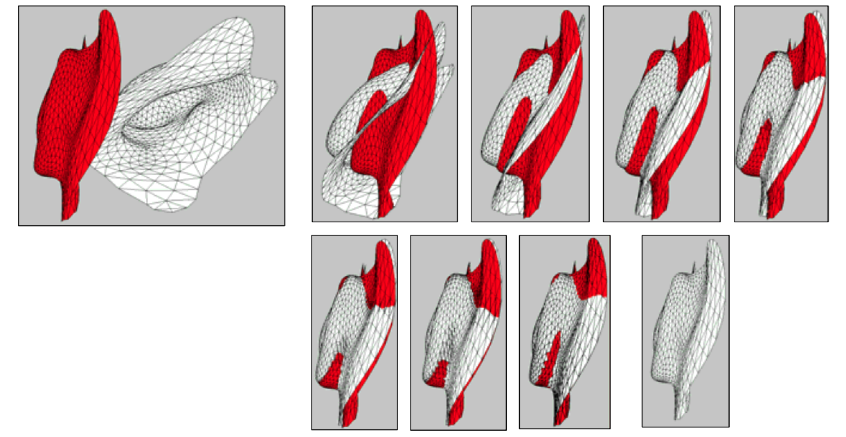
\includegraphics[width=\textwidth]{img/icp.png}
        \caption[Iteratívny výstup ICP algoritmu]{Iteratívny výstup ICP algoritmu~\cite{baiICPAlgorithmTheory2023}}\label{fig:icp}
      \end{figure}

      Ako už bolo spomenuté, existuje viacero variantov \acrshort{icp} algoritmu, ktoré je možné rozdeliť na základe viacerých kritérií~\cite{rusinkiewiczEfficientVariantsICP}:
      \begin{enumerate}
        \item Podľa typu minimalizačnej metriky:
        \begin{itemize}
          \item \emph{bod na bod}~--~najjednoduchšia verzia, minimalizuje euklidovskú vzdialenosť medzi korešpondujúcimi bodmi, vhodná pri povrchoch bez výraznej štruktúry
          \[\min_{\bm{R}, \bm{t}} \sum_i {\| \bm{R}\, \bm{s}_i + \bm{t} - \bm{d}_i \Vert}^2\]
          
          \item \emph{bod na plochu}~--~minimalizuje vzdialenosť od bodu k~rovine určenej normálou cieľového bodu, rýchlejšie konverguje, vhodný pre hladké povrchy
          \[ \min_{\bm{R}, \bm{t}} \sum_i {[ ( \bm{R}\, \bm{s}_i + \bm{t} - \bm{d}_i ) \cdot \bm{n}_i ]}^2 \]
          
          \item \emph{plocha na plochu}~--~predpokladá, že oba body majú definované normály a~minimalizuje vzdialenosť medzi dotyčnými rovinami. Používa sa napr.\ v~\acrshort{ndticp} alebo pokročilých \acrshort{slam} systémoch.
        \end{itemize}
        
        \item Podľa stratégia výberu korešpondencií:
        \begin{itemize}
          \item \emph{Brute-force nearest neighbor}~--~každý bod zo zdrojového mračna sa spáruje s~najbližším bodom v~cieľovom;
          \item \emph{Mutual nearest neighbor}~--~korešpondencia sa akceptuje iba vtedy, ak si oba body navzájom zodpovedajú ako najbližší sused;
          \item \emph{Color ICP}~--~pri výbere korešpondencií sa berie do úvahy aj podobnosť farby alebo intenzity;
          \item \emph{Feature-based ICP}~--~body sú doplnené o~deskriptory a~párujú sa na základe ich podobnosti.
        \end{itemize}
        
        \item Podľa robustnosti a~rýchlosti:
        \begin{itemize}
          \item \emph{Generalized ICP (G-ICP)}~--~spája metódy \emph{bod na bod} a~\emph{bod na plochu} pomocou modelovania pravdepodobnostného rozloženia bodov ako Gaussových distribúcií, vhodný pre zarovnávanie s~neistotou alebo nehomogenitou;
          \item \emph{Sparse ICP}~--~používa len podmnožinu bodov, čo šetrí výpočtový čas;
          \item \emph{Robust ICP}~--~používa robustné funkcie na potlačenie vplyvu odľahlých bodov.
          \item \emph{Color/Photometric ICP}~--~rozširuje ICP o~intenzitné alebo farebné informácie (vhodné pri RGB-D údajoch).
        \end{itemize}
        
        \item Iné pokročilé varianty:
        \begin{itemize}
          \item \emph{Normal Distributions Transform (NDT)}~--~Mračná bodov sa reprezentujú ako hustotné mapy (napr.\ v~bunkách), nie ako explicitné body;t
          \item \emph{Iterative Closest Line/Keypoint (ICLK)}~--~rozšírenia pre špecifické geometrie (čiary, body, hrany);
          \item \emph{KISS-ICP}~--~minimalistický robustný point-to-point ICP s~adaptívnym prahom a~robustným jadrom.
        \end{itemize}
      \end{enumerate}

      \paragraph{KISS ICP} \

      \noindent \acrshort{kissicp} predstavuje odľahčený variant klasického \acrshort{icp} algoritmu typu \emph{bod na bod} pre \acrshort{lo}. Cieľom autorov bolo preukázať, že dobre navrhnuté jednoduché komponenty dokážu prekonať zložité metódy. Systém má rádovo menej parametrov než iné metódy a~väčšinou nevyžaduje žiadne špecifické ladenie pre rôzne typy lidarov či prostredia~\cite{vizzoKISSICPDefensePointtoPoint2023}.
      
      Algoritmus prebieha v~štyroch základných krokoch. Najskôr sa vykonáva predikcia a~kompenzácia pohybu (angl.\ \emph{deskewing}), ktorej cieľom je kompenzovať rozptyl meraných bodov spôsobený pohybom lidaru počas skenovania a~predpovedať aktuálnu pozíciu registrovaných bodov. Namiesto fúzie s~kolesovou odometriou či \acrshort{imu} sa v~tomto prípade používa model konštantnej rýchlosti, a~to práve pre jeho jednoduchosť a~nezávislosť od ďalších senzorov či časovej synchronizácie. Model konštantnej rýchlosti predikuje aktuálnu polohu $\bm{T}_{pred,t}$ v~čase $t$ na základe rozdielu dvoch predošlých polôh definovaných pomocou translačného vektora a~rotačnej matice $\bm{T}_{t-1} = (\bm{R}_{t-1},\bm{t}_{t-1})$, $\bm{T}_{t-2} = (\bm{R}_{t-2}, \bm{t}_{t-2})$, pričom sa predpokladá, že translačná $\bm{v}_t$ a~rotačná rýchlosť $\bm{\omega}_t$ sa nemení.
      
      Predikovaná poloha a~z toho odvodené rýchlosti sa vypočítajú ako
      \begin{eqnarray}
        \bm{T}_{pred,t} &=&
        \begin{bmatrix}
          \bm{R}_{t-2}^{\top} \bm{R}_{t-1} & \bm{R}_{t-2}^{\top} (\bm{t}_{t-1} - \bm{t}_{t-2}) \\
          \bf 0 & 1
        \end{bmatrix},\\
        \bm{v}_t &=& \frac{\bm{R}_{t-2}^{\top}(\bm{t}_{t-1} - \bm{t}_{t-2})}{\Delta t}, \\
        \bm \omega_t &=& \frac{\mathrm{Log}(\bm R_{t-2}^{\top} \bm R_{t-1})}{\Delta t},
      \end{eqnarray}
      kde $\Delta t$ je čas akvizície lidarového snímku a~$\mathrm{Log}: SO(3) \rightarrow \mathbb{R}^3$ extrahuje osovo-uhlovú reprezentáciu rotácie. Ďalej sa predpokladá, že každý zosnímaný bod v~jednom skene $\bm{p_i} \in \mathcal{P}$ má relatívnu časovú značku v~rozmedzí $s_i \in \langle 0, \Delta t \rangle$, predstavujúcu uplynutý čas od začiatku snímania daného skenu. Korekcia pozície nameraných bodov je potom počítaná ako
      \begin{equation}
        \bm p_i^{\star} = \mathrm{Exp}(s_i\, \bm{\omega_t})\, \bm{p}_i + s_i \bm{v}_t,
      \end{equation}
      kde $\mathrm{Exp}: \mathbb{R}^3 \rightarrow SO(3)$ počíta rotačnú maticu z~osovo-uhlovej reprezentácie.
      
      Následne prebieha podvzorkovanie skenu pre zefektívnenie registrácie mračien. Mnohé iné prístupy vyhľadávajú význačné body, čo však pridáva ďalšiu vrstvu komplexnosti\@. \acrshort{kissicp} namiesto toho pracuje s~dvojkrokovým podvzorkovaním pomocou tvz.\ \emph{voxelov}, teda trojrozmerných buniek. Kým lokálna mapa je reprezentovaná voxelovou mriežkou s~rozlíšením $v \times v~\times v$, v~prvom kroku je vstupné mračno $\mathcal{P}^{\star}$ podvzorkované na voxely veľkosti $\alpha v$~--~čím vzniká mračno $\mathcal{P}^{\star}_{\mathrm{merge}}$ ktoré je neskôr použité na aktualizáciu mapy~--~a v~druhom kroku na voxely veľkosti $\beta v$ za vzniku mračna $\hat{\mathcal{P}}^{\star}$, ktoré sa použije na registráciu, platí $\alpha \in ( 0,1 \rangle$ a~$\beta \in \langle 1,2 \rangle$. Na rozdiel  od iných metód, v~ktorých sa súradnice voxelu určujú ako priemer všetkých bodov, ktoré obsahuje, v~tomto prípade sa použijú súradnice prvého bodu spadajúceho pod daný voxel, čím sa zamedzí vzniku diskretizačnej odchýlky, a~teda platí $\hat{\mathcal{P}}^{\star} \subseteq \mathcal{P}^{\star}$
      
      Ďalším krokom je určenie korešpondencií. Oproti klasickému \acrshort{icp}, kde sa porovnávajú dva po sebe nasledujúce snímky, \acrshort{kissicp} registruje vstupný snímok na celú lokálnu mapu, teda množinu všetkých v~minulosti registrovaných bodov. Následne sa voxelová mriežka mapy doplní o~novo registrované body s~tou podmienkou, že každý voxel má obmedzenú kapacitu, čo opäť cieli na celkovú efektivitu algoritmu. Na nastavenie prahovej hodnoty $\tau_t$ pre filtráciu odľahlých bodov sa využíva adaptívny výpočet. Ten zohľadňuje veľkosť zrýchlenia, ktoré spôsobuje nepresnosť predikcie v~predchádzajúcich krokoch.
      
      Proces získania globálneho odhadu polohy $\bm{T}_t$ začína transformáciou vstupného mračna pomocou predošlej polohy $\bm{T}_{t-1}$ a~predikcie $\bm{T}_{pred,t}$:
      \begin{equation}
        \mathcal{S} = \{ \bm{s}_i = \bm{T}_{t-1}\,\bm{T}_{pred,t}\,\bm{p}\, |\, \bm{p} \in \hat{\mathcal{P}}^{\star} \}
      \end{equation}

      V~každej iterácii $j$ sa získa množina korešpondencií medzi mračnom $\mathcal{S}$ a~lokálnou mapou $\mathcal{L} = \{\bm{q}_i\,|\,\bm{q}_i \in \mathbb{R}^3\}$ pomocou met=ody najbližšieho suseda s~prahovou hodnotou $\tau_t$. Odhad korekcie polohy sa potom počíta takto:
      \begin{equation}
        \Delta \bm{T}_{est,j} = \operatorname*{argmin}_{\bm{T}} \sum_{(s,q) \in \mathcal{C}(\tau_t)} \rho \left( \| \bm{T} \bm{s} - \bm{q} \Vert_2 \right),
      \end{equation}
      kde $\mathcal{C}(\tau_t)$ je množina korešpondencií najbližších susedov, ktorých vzdialenosť je menšia ako $\tau_t$ a~$\rho$ je Geman-McClure-ova robustná účelová funkcia. Vstupné body sú potom aktualizované pomocou vypočítanej korekcie, pričom celý postup sa opakuje až kým nie je splnená podmienka konvergencie, ktorou je $\Delta \bm{T}_{est,j} < \gamma$:
      \begin{equation}
        \{\bm{s}_i \leftarrow \Delta \bm{T}_{\mathrm{est},j} \bm{s}_i\, | \bm{s}_i \in \mathcal{S}\}
      \end{equation}
      
      Výsledkom je tak transformácia $\bm{T}_t = \Delta \bm{T}_{icp,t}\, \bm{T}_{t-1}\, \bm{T}_{\mathrm{pred, t}}$. Napokon, korekcia je aplikovaná na mračno $\mathcal{P}^{\star}_{\mathrm{merge}}$, ktoré je následne integrované do lokálnej mapy.

  \subsection{Inerčné snímače}    
    Inerčné snímače, resp.\ snímače zotrvačnosti slúžia na meranie vlastných stavových veličín~--~lineárnych a~uhlových rýchlostí a~zrýchlení robota. Nemerajú polohu priamo, ale v~kombinácii s~inými meraniami polohy môžu prispieť k~spresneniu odhadu polohy a~korekcii chýb iných meraní. Zaraďujeme tu gyroskopy, akcelerometre a~tiež magnetometre.

    \subsubsection{Gyroskopy}
      Gyroskopy zaznamenávajú zmeny v~natočení objektu, pričom poskytujú informáciu o~orientácii, príp.\ jej zmene vo všetkých osiach. Ich výstupom sú hodnoty vztiahnuté na pevný referenčný rámec. Väčšinou nie sú citlivé na elektromagnetické a~feromagnetické anomálie, takže na rozdiel od magnetických kompasov je ich využitie možné aj v~prostrediach bez prítomnosti geomagnetického poľa~\cite{duchonSnimaceMobilnejRobotike2012}.

      Gyroskopy je možné podľa technológie merania rozdeliť na mechanické a~optické. Podľa typu výstupných dát sa delia na derivačné a~integračné. Výstup derivačných gyroskopov je úmerný rotácii. Integračné gyroskopy sú schopné poskytnúť aj informáciu o~absolútnej polohe pomocou integrovania relatívnych hodnôt vztiahnutých na globálnu referenciu. Podobne ako u~odometrických snímačov, aj v~tomto prípade dochádza driftu. Na jeho potlačenie je možné využiť niektorú z~techník~\cite{duchonSnimaceMobilnejRobotike2012}:
      \begin{itemize}
        \item potlačenie šumu odstránením odľahlých hodnôt,
        \item potlačenie šumu aplikáciou metódy kĺzavého priemeru,
        \item aplikácia mierky na zmenu absolútnych uhlov,
        \item rekalibrácia gyroskopu vzorkovaním na strednú hodnotu,
        \item rekalibrácia gyroskopu vzorkovaním na minimálnu a~maximálnu hodnotu.
      \end{itemize}

      \paragraph{Mechanické gyroskopy} \

        \noindent Fungujú na princípe zákona zachovania hybnosti, pričom sa delia podľa toho, aký typ hybnosti využívajú~\cite{duchonSnimaceMobilnejRobotike2012}:
        \begin{enumerate}
          \item \emph{spojitá uhlová hybnosť}~--~gyroskopy so zotrvačníkom, čiastkové gyroskopy,
          \item \emph{kmitajúca uhlová rýchlosť}~--~gyroskopy s~torznou závesnou hmotou kmitajúcou na vlastnej frekvencii,
          \item \emph{spojitá lineárna hybnosť}~--~gyroskopy so stabilným tokom tekutiny, plazmy alebo elektrónov, ktoré majú tendenciu udržiavať vektor svojej rýchlosti pri otáčaní meracej platformy,
          \item \emph{kmitajúca lineárna hybnosť}~--~gyroskopy používajúce množinu kmitajúcej diskrétnej hmoty, pričom kmity sú vyvolané pozdĺž rovných čiar.
        \end{enumerate}

        Mechanický gyroskop na báze zotrvačníka pozostáva s~rýchlo rotujúceho kotúča alebo gule, ktorej väčšina hmoty je sústredená na vonkajšej periférii, a~to pre dosiahnutie vyššieho momentu zotrvačnosti. Rotujúce teleso je upevnené na dvoch na seba kolmých voľne rotujúcich osiach. Rotácia kotúča okolo prvej osi spôsobuje vznik momentu hybnosti $L$. Pri vzniknutí krútiaceho momentu $\tau$ na kolmú os (vplyvom vonkajších síl) dochádza k~zmene smeru momentu hybnosti prvej osi 
        \begin{equation}
          d\vec L = \vec \tau dt.
          \label{eq:precession1}
        \end{equation}
        Tejto jav sa nazýva \emph{precesia gyroskopu}~\cite{moebsUniversityPhysics2016}. Na obr.~\ref{sfig:precession} je bez straty na všeobecnosti znázornená situácia s~klasickým zotrvačníkom, v~ktorej je moment $\tau$ spôsobený tiažovým zrýchlením. Zo vzťahu~\ref{eq:precession1} je možné následne odvodiť, že veľkosť precesie $\omega_P$ je priamo úmerná krútiacemu momentu $\tau$~\cite{duchonSnimaceMobilnejRobotike2012}:
        \begin{equation}
          \tau = J \omega \Omega,
        \end{equation}
        kde $J$ je moment zotrvačnosti rotačného objektu a~$\omega$ je jeho uhlová rýchlosť, pričom platí $\omega_P \ll \omega$~\cite{moebsUniversityPhysics2016}. Typický príklad mechanického dvojosého gyroskopu je na obr.~\ref{sfig:gyroskop}.

        \begin{figure}[t!]
          \centering
          \begin{subfigure}[b]{0.45\textwidth}\centering
            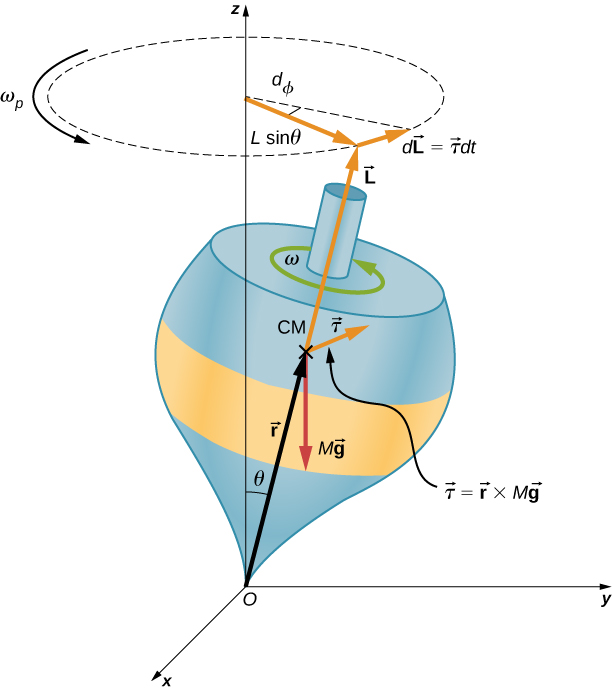
\includegraphics[width=\linewidth]{img/precession_gyroscope.jpg}
            \caption{Precesia gyroskopu so znázornením všetkých pôsobiacich síl a~momentov~\cite{moebsUniversityPhysics2016}}\label{sfig:precession}
          \end{subfigure}
          \hfill
          \begin{subfigure}[b]{0.5\textwidth}\centering
            \vspace*{\fill}
            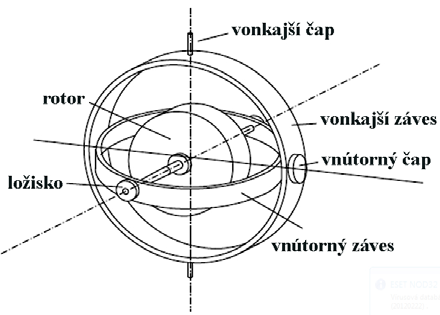
\includegraphics[width=\linewidth]{img/mechanicky_gyroskop.png}
            \vspace*{\fill}
            \caption{Dvojosý mechanický gyroskop so zotrvačníkom~\cite{duchonSnimaceMobilnejRobotike2012}}\label{sfig:gyroskop}
          \end{subfigure}
          \caption{Princíp gyroskopu~--~ilustrácia}
        \end{figure}

        Zvyškové trenie v~ložiskách gyroskopu, vonkajšie vplyvy a~malé nerovnováhy v~konštrukcii spôsobujú malú odchýlku v~zmysle dlhotrvajúcej stability, ktorá sa u~vysokokvalitných produktov pohybuje na úrovni okolo 0,1° za 6 hodín prevádzky~\cite{duchonSnimaceMobilnejRobotike2012}.

      \paragraph{Derivačné mechanické gyroskopy} \

        \noindent Fungujú na princípe mechanickej ladičky, ktorej vidlice vibrujú k~sebe a~od seba s~pevnou amplitúdou. Takýto snímač pozostáva z~páru vidlíc~--~riadenej a~snímacej. Rotácia okolo vertikálnej (torznej) osi vyvoláva vznik Coriolisových síl, pričom na každú z~vidlíc pôsobí sila
        \begin{equation}
          F = 2 m \Omega v_r,
        \end{equation}
        kde $F$ je Coriolisova sila pôsobiaca na vidlicu, $m$ je hmotnosť vidlice, $\Omega$ je vstupná rýchlosť otáčania a~$v_r$ je okamžitá uhlová rýchlosť vidlice. Coriolisove sily generujú rotačný moment, ktorý je priamo úmerný vstupnej uhlovej rýchlosti a~spôsobuje kmitanie snímacej vidlice, ktorá tak generuje signál~\cite{duchonSnimaceMobilnejRobotike2012}. Schematický náčrt takéhoto typu gyroskopu sa nachádza na obr.~\ref{fig:gyro_der}.

        \begin{figure}[t!]
          \centering
          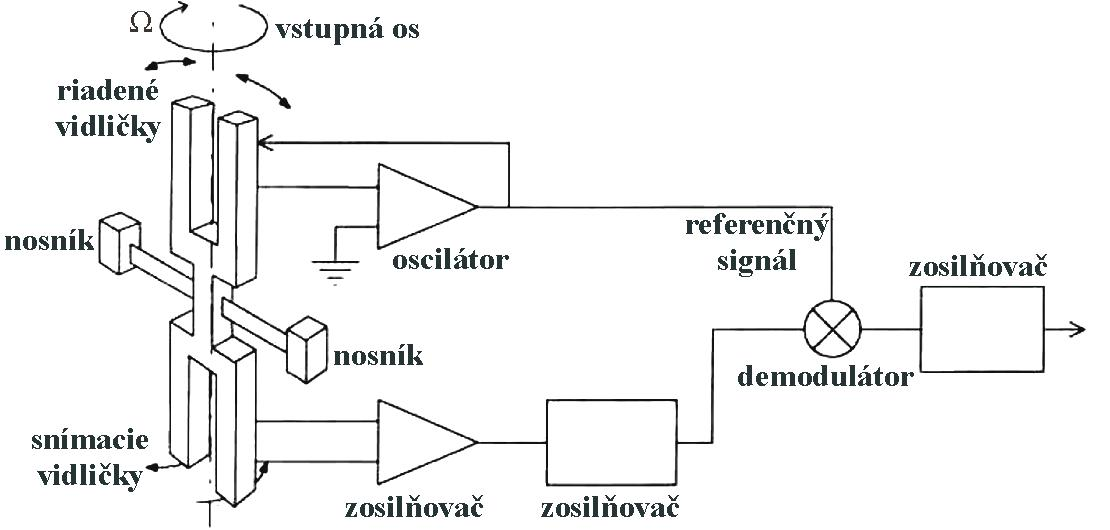
\includegraphics[width=\textwidth]{img/derivacny_gyroskop.jpg}
          \caption[Principiálna schéma gyroskopu Systron Donner GyroChip]{Principiálna schéma gyroskopu Systron Donner GyroChip~\cite{duchonSnimaceMobilnejRobotike2012}}\label{fig:gyro_der}
        \end{figure}

      \paragraph{Optické gyroskopy} \

      \noindent Uhlová rýchlosť je snímaná pomocou dvoch monochromatických svetelných lúčov, ktoré sú vysielané z~rovnakého zdroja do opačného smeru v~uzavretom kruhovom optickom vlákne. Lúče vytvárajú vo vnútri vlákna stojaté vlnenie s~kmitňami a~uzlami. Teoreticky by mal detektor s~každou otočkou laserového kruhu zaznamenať počet uzlov rovný dvojnásobku dráhy lúčov vydeleného ich vlnovou dĺžkou. V~skutočnosti však dosiahnutie takéhoto riešenia nie je možné kvôli vplyvu konštrukčných nedokonalostí~\cite{duchonSnimaceMobilnejRobotike2012}.

      Optické gyroskopy sa používajú v~nasledujúcich základných konfiguráciách~\cite{duchonSnimaceMobilnejRobotike2012}:
      \begin{itemize}
        \item \emph{Aktívne optické rezonátory}~--~využívajú tzv.\ Sagnacov efekt. Laserové lúče sú vysielané oproti sebe v~cyklickej dráhe. Pri rotácii dochádza k~predĺženiu dráhy jedného lúča a~skráteniu dráhy druhého. Rozdiel je priamoúmerný rotačnej rýchlosti. Ich nevýhodou je jav uzamknutia frekvencie pri nízkych rýchlostiach, ktorí súvisí s~periodickou moduláciou lasera v~spojení s~malým množstvom odrazov na reflexných plochách. Výsledkom je pásmo necitlivosti.
        \item \emph{Pasívne optické rezonátory}~--~používajú externý laser, čo zabraňuje vzniku uzamkntia frekvencie. Klasické implementácie používajú zrkadlové optické rezonátory. V~porovnaní s~aktívnymi majú menšie rozmery, vyššiu citlivosť aj robustnosť a~nižšiu cenu.
        \item \emph{Neriadené interferometrické gyroskopy z~optických vlákien (analóg)}~--~vďaka využitiu optických vlákien je možné zmenšenie rozmerov a~predĺženie dráhy lúčov, z~čoho vyplýva zvýšenie rozlíšenia a~znížené výrobné náklady. Medzi výhody tiež patrí vysoká tolerancia na vibrácie a~otrasy, necitlivosť na gravitačné efekty, rýchly štart a~dobrá citlivosť. Nevýhodami sú veľká dĺžka optického vlákna, obmedzený dynamický rozsah a~odchýlky kvôli použitým analógovým komponentom. Používajú sa zväčša v~jednoduchších aplikáciách vyžadujúcich strednú presnosť.
        \item \emph{Riadené interferometrické gyroskopy z~optických vlákien (digitál)}~--~citlivý prvok merajúci fázový posun nevyužíva Sagnacov efekt, ale pracujú s~fázovým posunom lúčov $\Delta \phi = 0$. Ich výhodou je veľká presnosť, nezávislosť od intenzity svetla vysielaného v~gyroskope, nezávislosť od zosilnení jednotlivých komponentov gyroskopu a~lineárnosť a~stabilita závislá len od nerecipročného fázového vysielača. Drift tohto typu gyroskopov sa pohybuje v~rozmedzí 0,0001--0,01°/hod.
        \item \emph{Rezonančné gyroskopy s~optickými vláknami}~--~princíp ich činnosti bol odvodený od pasívnych optických rezonátorov. Výhodami sú vysoká spoľahlivosť, dlhá životnosť, rýchly štart a~malá hmotnosť. Nevýhodou je nutnosť použitia vysoko koherentného zdroja svetla a~extrémne bezstratových komponentov optického vlákna.
      \end{itemize}
    
    \subsubsection{Akcelerometre}

      Zrýchlenie je vektorová fyzikálna veličina popisujúca zmenu vektoru rýchlosti~--~jeho veľkosti alebo smeru. Z~Newtonových pohybových zákonov je známe, že teleso mení rýchlosť len keď na neho pôsobí sila (I.\ zákon) a~táto sila spôsobuje jej úmerné zrýchlenie (II.\ zákon). Akcelerometre sú snímače vyvinuté na zaznamenanie síl na nich pôsobiacich, teda výstupom z~nich je signál priamo úmerný akcelerácii.
    
      Na zaznamenanie rôznych fyzikálnych síl sa v~akcelerometroch využívajú rôzne citlivé elementy. Podľa spôsobu toho sa akcelerometre delia na\cite{duchonSnimaceMobilnejRobotike2012}:
      \begin{itemize}
        \item \emph{mechanické}~--~(obr.~\ref{sfig:mech_acc}) merajú zrýchlenie pomocou pružiny, pričom využívajú Newtonov druhý pohybový zákon a~Hookov zákon opisujúci tuhosť pružiny. Zrýchlenie spôsobuje deformáciu pružiny, ktorá je úmerná zrýchleniu;
        \item \emph{piezoelektrické}~--~(obr.~\ref{sfig:pies_acc}) využívajú piezoelektrický efekt~--~pri deformácii keramického kryštálu sa pôsobením zrýchlenia generuje elektrický náboj, ktorý je úmerný sile. Pracujú najlepšie v~stredných a~vysokých frekvenciách;
        \item \emph{piezorezistívne}~--~sú založené na zmene elektrického odporu pri mechanickom namáhaní piezorezistívneho materiálu. Umožňujú merať aj konštantné zrýchlenie (0 Hz), čo ich odlišuje od piezoelektrického typu;
        \item \emph{tepelné}~--~(obr.~\ref{sfig:temp_acc}) merajú zrýchlenie na základe zmien rozloženia teploty v~plyne ohrievanom výhrevným telesom. Neobsahujú pohyblivé časti a~sú veľmi odolné, ale citlivé na zmeny okolitej teploty;
        \item \emph{elektromechanické}~--~obsahujú pohyblivý mechanický prvok spojený s~elektrickou časťou (napr.\ kondenzátorom). Zrýchlenie spôsobuje pohyb prvku, čo vedie k~zmene elektrickej veličiny~--~najčastejšie kapacity.
      \end{itemize}

      \begin{figure}[b!]
        \centering
        \begin{subfigure}[b]{0.32\textwidth}
          \centering
          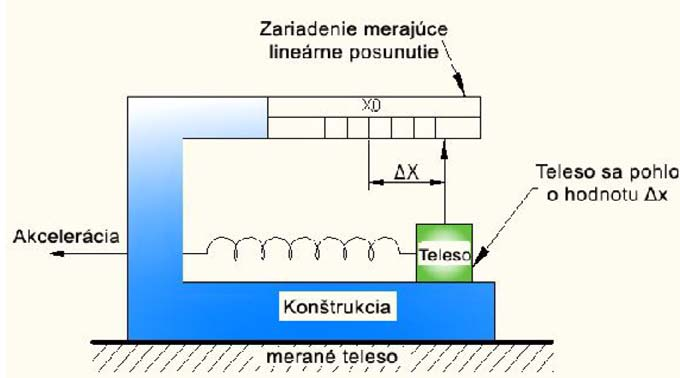
\includegraphics[height=0.115\textheight]{img/mechanicky_akcelerometer.png}
          \caption{mechanický}\label{sfig:mech_acc}
        \end{subfigure}
        \hfill
        \begin{subfigure}[b]{0.32\textwidth}
          \centering
          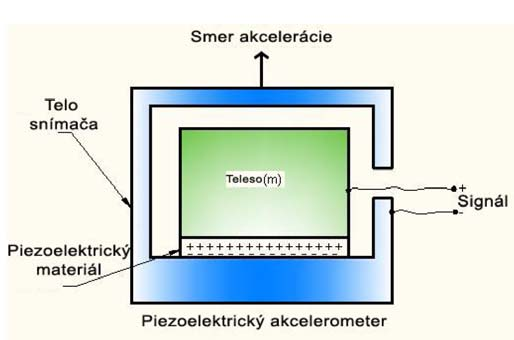
\includegraphics[height=0.125\textheight]{img/piezoelektricky_akcelerometer.png}
          \caption{piezoelektrický}\label{sfig:pies_acc}
        \end{subfigure}
        \hfill
        \begin{subfigure}[b]{0.32\textwidth}
          \centering
          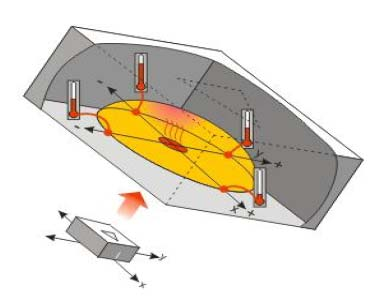
\includegraphics[height=0.125\textheight]{img/tepelny_akcelerometer.png}
          \caption{tepelný}\label{sfig:temp_acc}
        \end{subfigure}
        \hfill
        \caption[Štruktúra a~princíp merania rôznych typov akcelerometrov]{Štruktúra a~princíp merania rôznych typov akcelerometrov~\cite{duchonSnimaceMobilnejRobotike2012}}\label{fig:acc}
      \end{figure}

      Akcelerometre sú schopné zaznamenať zrýchlenie len v~jednej osi. Pre meranie trojrozmerného zrýchlenia sa používajú systémy zložené z~kombinácie troch vzájomne kolmých akcelerometrov. Ich najväčšou nevýhodou je vysoká citlivosť na  vibrácie mechanických častí robota ako aj na rôzne parazitné zrýchlenia. Tento problém sa obvykle rieši zvýšením pomeru dĺžky citlivého elementu k~jeho šírke v~požadovanom smere~\cite{duchonSnimaceMobilnejRobotike2012}.

    \subsubsection{Magnetometre}

      Magnetometre (magnetické kompasy) sú prístroje, ktoré sú schopné zaznamenať magnetické pole Zeme. Na základe ich meraní je možné stanoviť orientáciu robota. Magnetické kompasy využívané v~mobilnej robotike sa delia na~\cite{duchonSnimaceMobilnejRobotike2012}:
      \begin{itemize}
        \item \emph{mechanické magnetické kompasy}~--~tradičné kompasy s~otočným diskom v~kvapaline, často upevnené na guľovom závese na kompenzáciu pohybu. Okolité magnetické anomálie sa potláčajú pomocou nastaviteľných permanentných magnetov. Sú náchylné na odchýlky z~externých zdrojov.
        \item \emph{kompasy s~magnetickou indukčnou sondou}~--~používajú dvojicu navzájom kolmých cievok s~feritovým jadrom. Merajú horizontálnu zložku magnetického poľa pomocou sínusových výstupov. Ich výhodou je nízka spotreba, odolnosť voči otrasom a~rýchly štart. Nevýhodou je citlivosť na magnetické anomálie, ktorú možno potlačiť spojením s~gyroskopom.
        \item \emph{magneticko-indukčné kompasy}~--~využívajú solenoid ako súčasť L/R oscilátora, kde frekvencia závisí od induktancie ovplyvnenej magnetickým poľom. Elektronika je jednoduchšia a~spotreba energie nižšia ako pri kompasoch na báze magnetickej indukčnej sondy. Výstup má digitálny charakter.
        \item \emph{kompasy na báze Hallovho efektu}~--~merajú rozdiely napätí v~polovodiči so stálym prúdom pri prítomnosti magnetického poľa. Dvojica kolmých senzorov umožňuje výpočet uhla natočenia. Sú lacné, ale s~nízkym rozlíšením a~silným vplyvom vnútorných chýb, čo vyžaduje filtrovanie a~znižuje šírku pásma.
        \item \emph{magneticko-rezistívne kompasy}~--~Využívajú zmenu odporu anizotropného materiálu pri zmene smeru magnetizácie. Umožňujú veľmi citlivé meranie natočenia, sú vhodnú najmä pre aplikácie vyžadujúce vysokú presnosť.
        \item \emph{magneticko-elastické kompasy}~--~sú založené na zmene Youngovho modulu magneticko-striktívnych materiálov pri pôsobení magnetického poľa. Meranie je založené na detekcii deformácie materiálu vyžaduje zliatiny s~vysokou magnetostrikciou.
      \end{itemize}

    \subsubsection{IMU}
      Inerčná meracia jednotka (niekedy nazývaná aj inerčná referenčná jednotka alebo pohybová referenčná jednotka, skr.\ \acrshort{imu}, alebo tiež inerčný navigačný systém, skr.\ \acrshort{ins}) je zväčša elektromechanické alebo polovodičové zariadenie, ktoré obsahuje kombináciu viacerých senzorov (zvyčajne akcelerometrov a~gyroskopov, ale tiež magnetometrov a~tlakových senzorov) schopných merať pohyb, teda lineárne a~uhlové zrýchlenia, uhlové rýchlosti, príp.\ aj orientáciu, a~to vo všetkých troch osiach. Je schopná zaznamenať zotrvačné sily a~a transformovať ich na výstupné údaje, ktoré opisujú pohyb objektu~\cite{InertialMeasurementUnit2023}.

      Najpoužívanejšou konštrukčnou technológiou pre \acrshort{imu} je \acrshort{mems}. Sú to miniatúrne zariadenia s~veľkosťou rádovo v~mikrometroch, ktoré sú tvorené kombináciou elektrických a~mechanických prvkov tvorených z~rôznych materiálov (napr.\ kremík, polyméry, kov). Existujú rôzne typy \acrshort{mems} komponentov, od jednoduchých prepínačov až po mimoriadne zložité elektromechanické systémy s~viacerými integrovanými snímačmi a~mikroelektronikou~\cite{InertialMeasurementUnit2023}.

      Výhody použitia \acrshort{mems} technológie spočívajú najmä v~mimoriadne malej veľkosti a~hmotnosti komponentov v~kombinácii s~nízkou spotrebou energie. Vďaka tomu je možné takéto snímače umiestniť na malých plošných spojoch do kompaktných puzdier a~sú vhodné na umiestnenie v~mobilných robotoch, ktoré majú obvykle značné priestorové aj napájacie obmedzenia. Jednotlivé komponenty, materiály a~konštrukčné techniky zabezpečujú vysokú spoľahlivosť a~dlhú životnosť, pričom tieto parametre sú stále predmetom neustáleho zdokonaľovania sa~\cite{InertialMeasurementUnit2023}.

      Na druhú stranu, pre správnu interpretáciu výstupných dát z~\acrshort{imu} je potrebné ďalšie spracovanie, a~to za účelom odstránenia tiažového zrýchlenia a~tiež filtrácie šumu meraní, ktorý pri vysokej citlivosti snímačov môže spôsobiť vznik drift odhadu polohy. Vzhľadom na vysokú mieru šumu meraní sa \acrshort{imu} senzory väčšinou nepoužívajú samostatne, ale vo fúzii s~inými senzormi. Vďaka skutočnosti, že meria reálne fyzikálne veličiny na základe priameho vplyvu zotrvačných síl, údaje z~nej sú nápomocné v~kombinácii so snímačmi, ktoré merajú polohu na základe iných metód odhadu (kamera, lidar, \acrshort{gps}, a~i.) a~u~ktorých zvykne dochádzať napríklad ku skokovým zmenám odhadu, ktoré fyzikálne nie sú možné. Aplikácie, v ktorých sa na fúziu lokalizácie využíva \acrshort{imu} v kombinácii s inými senzormi uvádzame v častiach práce venovaných daným senzorom, preto ich na tomto mieste už špeciálne uvádzať nebudeme. Algoritmy, ktoré sa zaoberajú fúziou dát z~viacerých snímačov budeme bližšie rozoberať v~ďalších častiach práce.

      % Open GINS

\section{Externé lokalizačné systémy}\label{sec:absolute}

  Pokiaľ na lokalizáciu robota používame zariadenia umiestnené mimo neho, hovoríme o~externých lokalizačných systémoch. Na určenie polohy robota sa najčastejšie využívajú princípy trilaterácie na základe merania vzdialeností k referenčným objektom (napr.\ pomocou \acrshort{tof} merania), príp.\ triangulácie na základe určenia smerových vektorov medzi robotom a~referenciami. Dôležitým predpokladom pre využitie externej lokalizácie je časová synchronizáciami medzi jednotlivými prvkami lokalizačného systému.
  
  Najpoužívanejšou skupinou externých lokalizačných systémov najmä pre exteriérové aplikácie sú \acrshort{gnss}. Tie však dosahujú obmedzenú presnosť a~v~interiéroch sú zvyčajne nepoužiteľné. Externá lokalizácia vo vnútornom prostredí je s~obľubou využívaná najmä v~priemyselnom odvetví, kde je pracovný priestor robota dobre známy a~relatívne nemenný. Využívajú sa rôzne kombinácie pasívnych a~aktívnych prvkov na referenčných pozíciách, z ktorých sa určuje aktuálna poloha robota. Výhodou je dlhodobá stabilita takejto lokalizácie. 

  \subsection{GNSS systémy}
    
    Globálne navigačné satelitné systémy (\acrshort{gnss}) sú systémy slúžiace na určenie polohy, rýchlosti a~času~\cite{duchonSnimaceMobilnejRobotike2012}. Pozostávajú zo zoskupení satelitov, ktoré neustále vysielajú informáciu o~svojej polohe a~čase, zo siete pozemných staníc a~z prijímačov, ktoré vypočítavajú polohu na zemi pomocou trilaterácie. Používajú sa vo všetkých formách dopravy: na vesmírnych staniciach, v~letectve, námornej doprave, železničnej doprave, cestnej doprave a~hromadnej doprave~\cite{GNSS}.

    V~súčasnosti existuje niekoľko globálnych systémov~\cite{WhatGNSS}:
    \begin{itemize}
      \item \acrshort{gps} (Spojené štáty americké),
      \item \acrshort{glonass} (Ruská federácia),
      \item GALILEO (Európska Únia),
      \item COMPASS/Bei-Dou (Čína).
    \end{itemize}
    
    Okrem nich sú v~priebežnom vývoji aj ďalšie regionálne systémy, ako napríklad indický \acrshort{irnss} a~japonský \acrshort{qzss}. V~momente dokončenia všetkých týchto systémov bude pre užívateľov k~dispozícii dokopy viac než sto satelitov. Jednou z~najaktuálnejších tém v~rámci oblasti \acrshort{gnss} je zabezpečenie interoperability medzi globálnymi systémami, čo by umožnilo užívateľom prijímať a~spracúvať signál z~viacerých satelitných systémov pomocou jedného zariadenia~\cite{GNSS}.

    Výkonnosť \acrshort{gnss} sa hodnotí podľa štyroch kritérií~\cite{WhatGNSS}:
    \begin{enumerate}
      \item \emph{presnosť}~--~rozdiel medzi nameranou a~skutočnou polohou, rýchlosťou alebo časom prijímača,
      \item \emph{integrita}~--~schopnosť systému poskytnúť určenú mieru spoľahlivosti a~v prípade poruchy v~údajoch o~polohe vydať varovanie,
      \item \emph{kontinuita}~--~schopnosť systému fungovať bez prerušenia,
      \item \emph{dostupnosť}~--~percentuálny podiel času, počas ktorého signál spĺňa uvedené kritériá presnosti, integrity a~kontinuity.
    \end{enumerate}

    Túto výkonnosť je možné zlepšiť pomocou regionálnych satelitných augmentačných systémov (\acrshort{sbas}). Ich kombinácia s~overenými pozemnými technológiami, ako je inerciálna navigácia, prináša možnosti novým aplikáciám, ktoré nevyžadujú len presnosť, ale predovšetkým spoľahlivosť a~integritu.

    Medzi hlavné výhody \acrshort{gnss} patria vysoká presnosť, údaje v~jednotnom svetovom súradnicovom systéme \acrshort{wgs} a~nezávislosť na počasí či fáze dňa. Nevýhodami sú nemožnosť využitia v~podzemí, vo vode aj v~interiéroch s~hrubými či početnými stenami, horšia presnosť v~prostrediach s~menšou viditeľnosťou na oblohu (napr.\ oblasti husto zastavané vysokými budovami, lesy, údolia) či možnosť rušenia signálu externým zdrojom~\cite{duchonSnimaceMobilnejRobotike2012}.
    
    \subsubsection{Princíp činnosti}

      Princíp určovania polohy pomocou \acrshort{gnss} spočíva v~meraní času letu rádiového signálu z~družíc. Každý satelit vysiela svoje identifikačné údaje, polohu a~časovú značku. Prijímač vypočíta odhad vzdialenosti družice na základe rozdielu medzi časom vyslania a~prijatia signálu. Polohu meraného bodu je možné určiť vyhodnotením takéhoto signálu z~viacerých satelitov. Z~geometrického hľadiska by na určenie trojrozmernej polohy mal stačiť prienik vzdialeností troch družíc. Keďže ale nie je možné zaručiť presnú synchronizáciu hodín prijímača, je potrebný údaj z~ešte aspoň jedného satelitu, čím vznikne viacero bodov prieniku, tzv.\ \emph{pseudovzdialeností}. Čas prijímača je následne posúvaný tak, aby tieto body splynuli do jediného, čím vzniká výsledné meranie polohy (viď obr.~\ref{fig:gps}). Pre dosiahnutie vyššej presnosti potrebné poznať polohy čo najväčšieho počtu vhodne rozložených družíc~\cite{duchonSnimaceMobilnejRobotike2012}.

      \begin{figure}[t!]
        \centering
        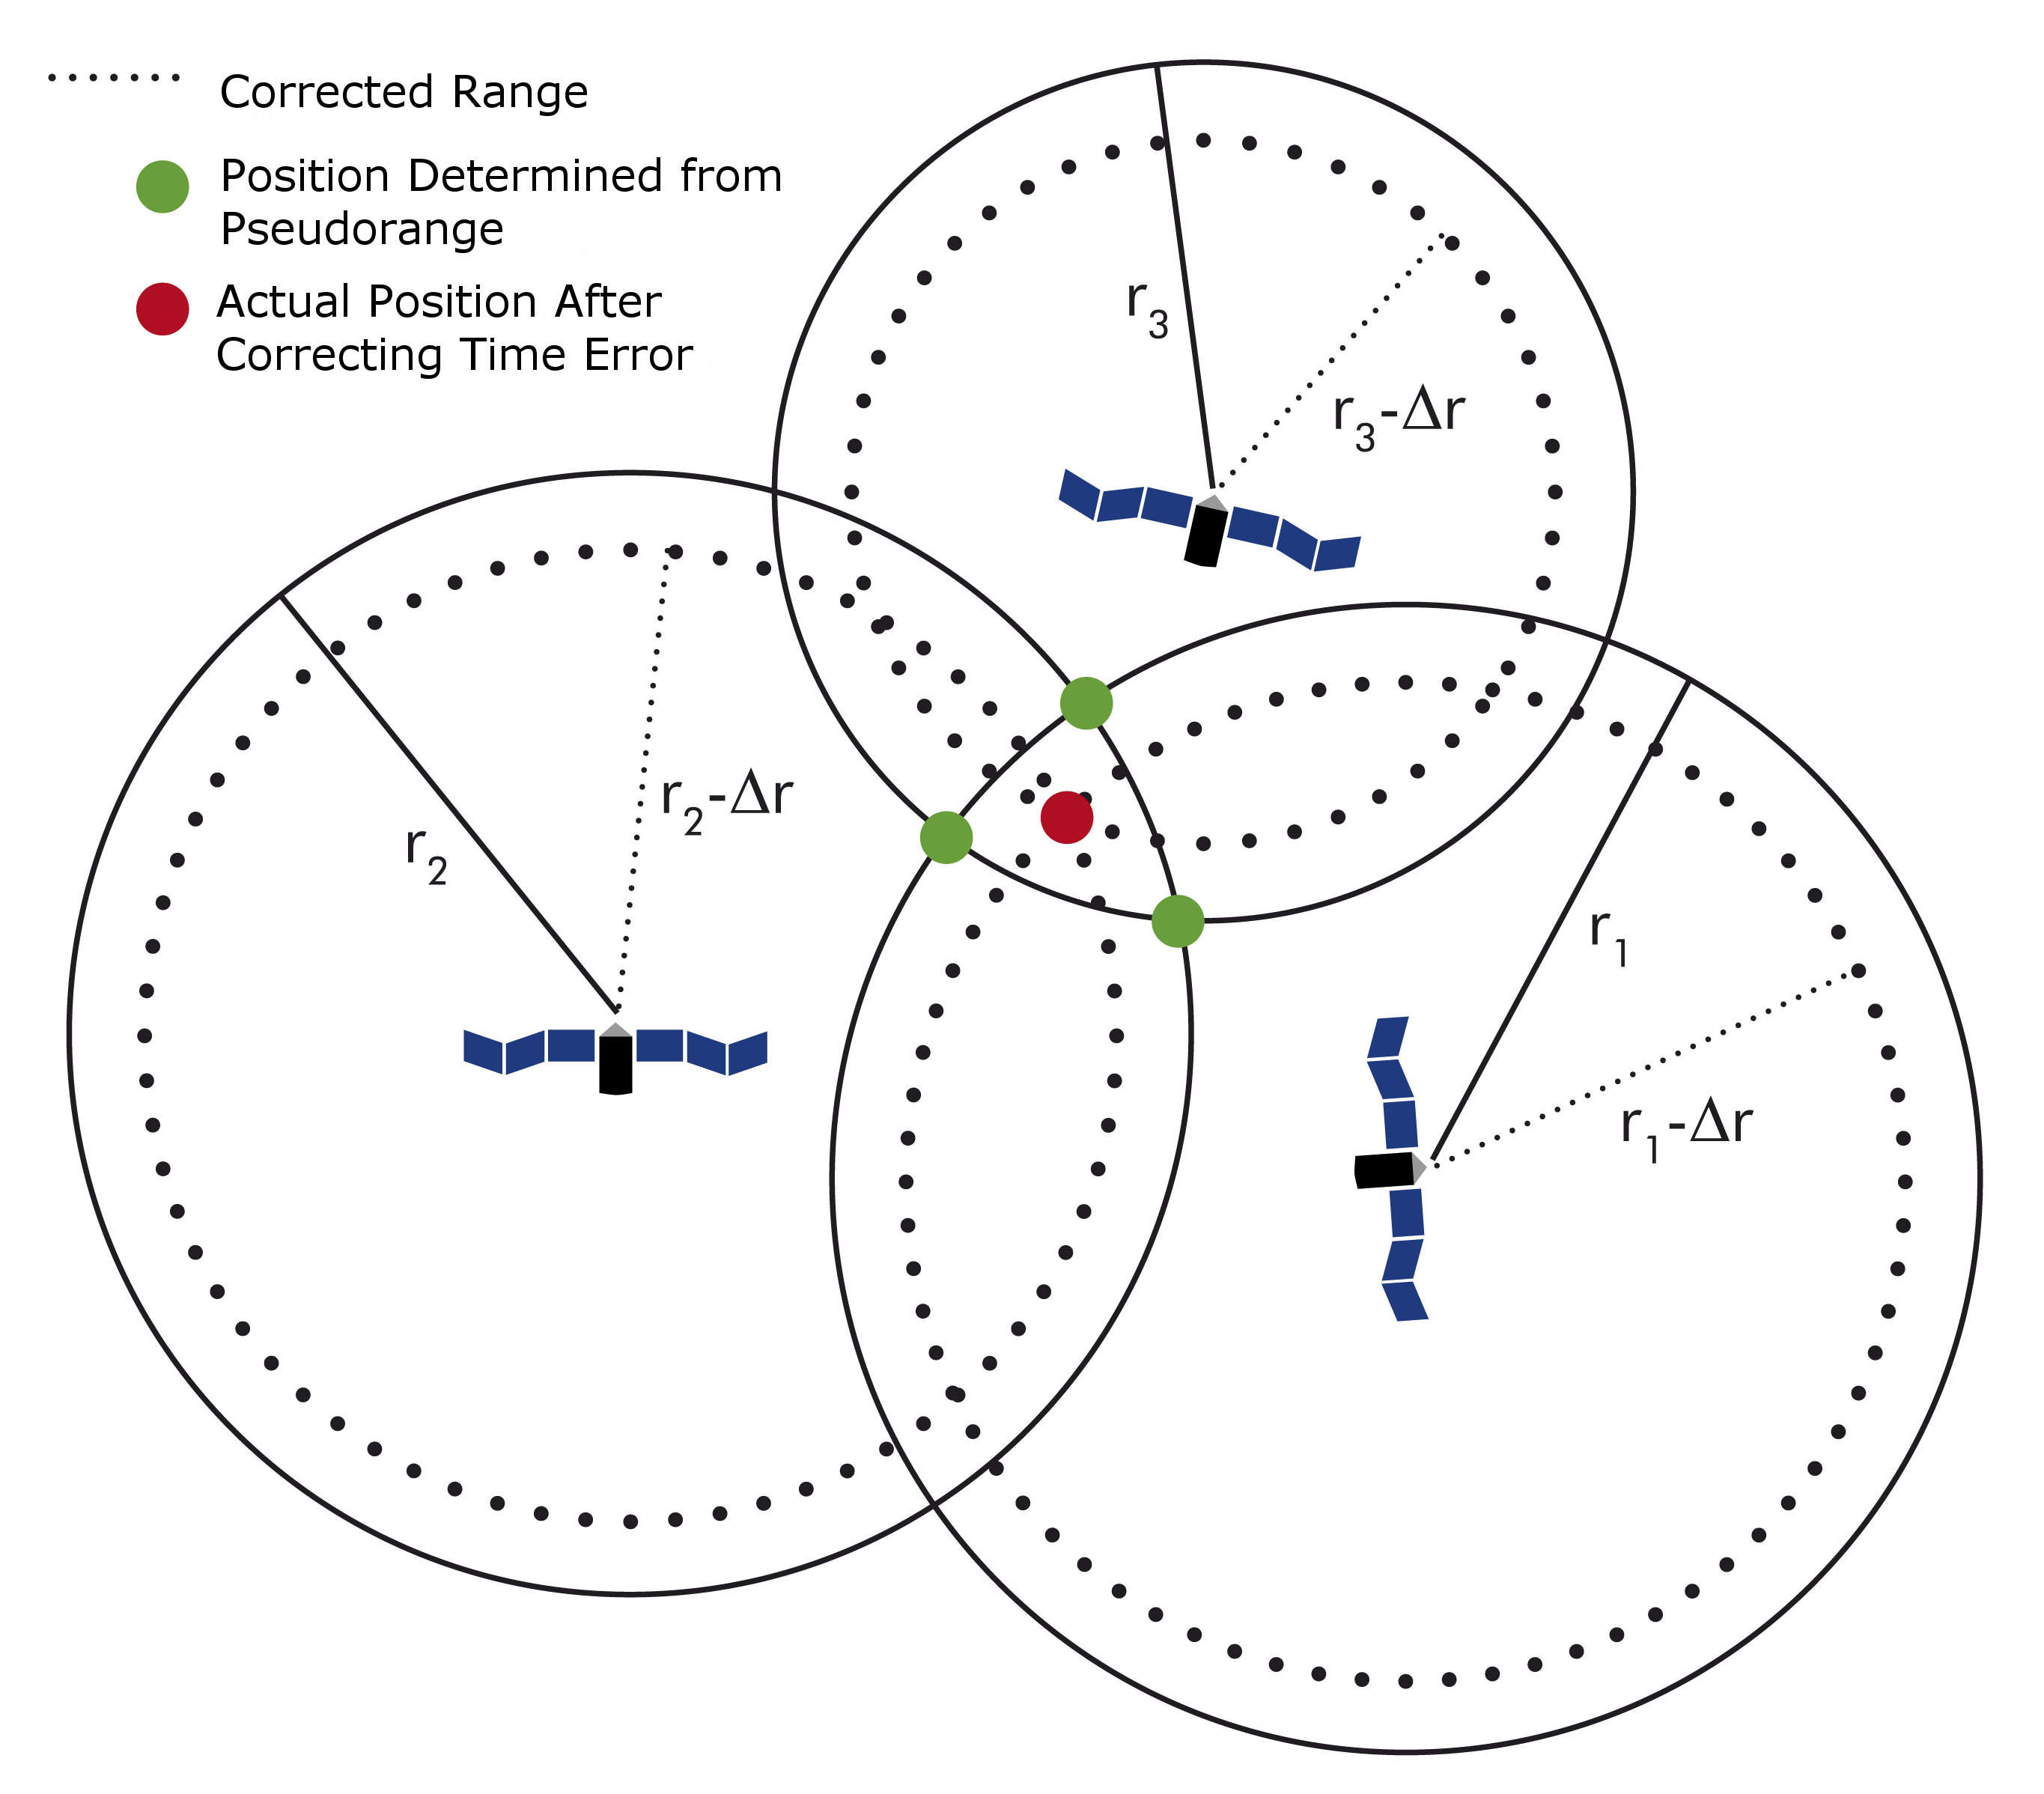
\includegraphics[width=0.7\textwidth]{img/GPS_trilateration.png}
        \caption[Princíp lokalizácie pomocou GNSS]{Princíp lokalizácie pomocou GNSS. $r_1, r_2, r_3$ sú pseudovzdialenosti, $\Delta r$ je odchýlka merania vzdialenosti.~\cite{HowDoesGPS2025}}\label{fig:gps}
      \end{figure}

    \subsubsection{Chyby GPS}\label{ssec:gps_error}
      Merania \acrshort{gps} sú sprevádzané niekoľkými typmi chýb~\cite{duchonSnimaceMobilnejRobotike2012}:
      \begin{itemize}
        \item \emph{Geometria rozloženia satelitov}~--~pokiaľ aktuálne viditeľné satelity nie sú rovnomerne rozložené po celej oblohe, môže dojsť k~nepresnej triangulácii, a~teda aj k~chybe odhadu polohy. Viditeľnosť satelitov negatívne ovplyvňuje aj meranie vnútri vozidla, v~blízkosti vysokých budov či v~členitom teréne. Tento typ chyby vyjadruje parameter zníženia presnosti (\acrshort{dop}).
        
        \item \emph{Atmosférické efekty}~--~zemská atmosféra ovplyvňuje \acrshort{gps} signály dvomi hlavnými vrstvami: troposférou a~ionosférou. Troposféra ako elektricky neutrálne prostredie spôsobuje nedisperzné odchýlky závislé od teploty, tlaku a~vlhkosti, ktoré rovnomerne postihujú fázové aj kódové \acrshort{gps} merania. Ionosféra je elektricky aktívna vrstva s~voľnými elektrónmi a~iónmi, kde dochádza k~odrazu a~útlmu rádiových vĺn, najmä v~dôsledku interakcie s~neutrálnymi molekulami. Jej účinky závisia od slnečnej aktivity a~polohy v~atmosfére a~spôsobujú spomalenie elektromagnetických vĺn úmerné k~prevrátenej hodnote kvadrátu ich frekvencie. Vplyv ionosféry možno čiastočne eliminovať porovnaním signálov na rôznych frekvenciách, čo využívajú napríklad vojenské \acrshort{gps} prijímače pracujúce.
        
        \item \emph{Efekt viaccestného šírenia sa signálu (angl.\ multipath)}~--~nastáva, keď sa \acrshort{gps} signál odrazí od objektov v~okolí prijímača a~dorazí k~nemu oneskorene. Tieto odrazené signály predlžujú dráhu, ktorú signál prejde, čo vedie k~chybám v~určení polohy~--~typicky v~rozsahu niekoľkých metrov\@. \acrshort{gps} satelity vysielajú signál v~širokom kuželi, takže odrazy sú bežné najmä v~mestskom alebo členitom prostredí. Na zníženie tohto efektu sa používajú antény so špeciálnou konštrukciou (napr.\ s~ochranným tanierom), pokročilé technológie v~prijímači a~efektívne metódy spracovania signálu. Tieto opatrenia znižujú príjem odrazených signálov, čím zlepšujú presnosť určenia polohy.
        
        \item \emph{Relativistické efekty}~--~zohrávajú významnú úlohu pri určovaní polohy pomocou \acrshort{gps}, najmä kvôli veľkej rýchlosti a~výške družíc. Zmeny frekvencie signálu v~dôsledku rýchlosti pohybu družíc (Dopplerov jav) a~rozdiely v~priebehu času spôsobené gravitáciou (dilatácia času) ovplyvňujú presnosť meraní. Tieto efekty sú dôsledkom špeciálnej aj všeobecnej teórie relativity a~musia byť zahrnuté do výpočtov polohy. Bez ich korekcie by chyba v~určovaní času spôsobila výrazné chyby v~polohe, až rádovo kilometre denne. Preto sú súčasťou rovníc používaných v~\acrshort{gps} prijímačoch aj korekcie na relativistické poruchy dráh družíc a~šírenia signálu.
        
        \item \emph{Ďalšie chyby \acrshort{gps}}
        \begin{itemize}
          \item nepresnosť hodín v~\acrshort{gps} prijímači (prijímač nemôže obsahovať atómové hodiny, odstránenie chyby sa rieši použitím signálu z~viacerých satelitov),
          \item nepresné určenie parametrov dráhy družice (tzv.\ ephemeris error),
          \item počet viditeľných satelitov (pre väčšiu presnosť merania je potrebné mať väčší počet viditeľných satelitov).
        \end{itemize}
      \end{itemize}

    \subsubsection{Augmentačné systémy}
      Spomenuté chyby \acrshort{gps} meraní je možné v~rôznej miere potlačiť pomocou systémov so zvýšenou presnosťou. Tie bývajú častou voľbou aj v~prípade mnohých robotických aplikácií, pre potreby ktorých je presnosť meraní pomocou \acrshort{gnss} nedostatočná~\cite{duchonSnimaceMobilnejRobotike2012}.
    
      \paragraph{Inertial Navigation System (INS)} \
      
      \noindent Pridaním \acrshort{ins} ku \acrshort{gps} je možné dosiahnuť presnosť v~rozsahu približne jedného metra. Výstup z~oboch systémov býva porovnávaný obvykle pomocou Kalmanovho filtra, ktorý poskytuje najviac pravdepodobné meranie.
    
      \paragraph{Differential GPS (DGPS)} \
      
      \noindent Potrebné sú dva \acrshort{gps} prijímače, z~ktorých jeden sa nachádza na geodeticky vymeranej polohe. Využíva sa skutočnosť, že blízke prijímače majú vysokú koreláciu chýb. Referenčná stanica vypočítava a~vysiela korekcie na základe rozdielov medzi očakávanými a~nameranými údajmi zo všetkých viditeľných družíc. V~prijímači užívateľa \acrshort{dgps} je korekčný údaj využitý na opravu merania. Použitím \acrshort{dgps} môže užívateľ získať presnosť určovania polohy v~reálnom čase na úrovni desiatok centimetrov až metrov, v~závislosti od vzdialenosti od referenčnej stanice.

      \paragraph{Real-Time Kinematic (RTK) GPS} \
      
      \noindent \acrshort{rtk} je vysoko presná technológia pre lokalizáciu a~navigáciu, využívaná v~širokom spektre aplikácií od prieskumu a~mapovania, cez poľnohospodárstvo až po stavebníctvo. Funguje, podobne než \acrshort{dgps}, na kombinácii referenčnej stanice a~užívateľského prijímača. Na rozdiel od \acrshort{dgps} však referenčná stanica uskutočňuje aj meranie nosnej fázy signálu. Prijímač potom odlišnosti v~nosnej fáze vyhodnocuje, čo dramaticky zvyšuje presnosť merania polohy~\autocite{RTKGPSTechnologyPrecise}.

      \paragraph{Wide Area Augmentation System (WAAS)} \
      
      \noindent Systém \acrshort{waas} poskytuje extrémne vysokú presnosť lokalizácie, využiteľnú najmä v~leteckej doprave. Pozostáva z~38 referenčných staníc (\acrshort{wrs}), 3 hlavných staníc (\acrshort{wms}), 3 geostacionárnych družíc a~6 pozemných vysielacích staníc. Referenčné stanice slúžia na prijímanie signálu \acrshort{gps}\@. Ich polohy sú zvolené tak, aby bolo možné zachytiť akékoľvek chyby v~signáloch \acrshort{gps}\@. Informácie z~\acrshort{wrs} sa posielajú do \acrshort{wms}, ktoré vysielajú správy pre užívateľov s~frekvenciou 1 Hz. Tieto správy umožňujú významnú korekciu \acrshort{gps} meraní na strane užívateľa\@. \acrshort{wms} vysiela správy aj na pozemné vysielacie stanice, odkiaľ sú prenášané k~navigačným zariadeniam na geostacionárnych komunikačných satelitoch. Tie následne vysielajú signál podobný \acrshort{gps}, ktorý môžu prijímače využiť spolu s~korekčnými údajmi na spresnenie lokalizácie. Systém \acrshort{waas} je dostupný v~rámci \acrshort{nas}~\cite{SatelliteNavigationWAAS}. V~Európe funguje na podobnom princípe systém \textbf{\acrshort{egnos}}~\cite{EGNOS}.

  \subsection{UWB systémy}
    Ultra-širokopásmové (\acrshort{uwb}) systémy predstavujú modernú bezdrôtovú technológiu využívajúcu veľmi krátke rádiové impulzy (rádovo v~nanosekundách) v~širokom frekvenčnom pásme (typicky 3,1~--~10,6\ GHz) s~nízkou spektrálnou hustotou výkonu, vďaka čomu má malú spotrebu energie. Je schopná prenášať dáta vysokou rýchlosťou (do 100 Mb/s) na krátku vzdialenosť. Používanie krátkych impulzných vĺn namiesto kontinuálneho šírenia signálu znižuje riziko vzniku \uv{multipath} efektu (spomínaného v~časti~\ref{ssec:gps_error}) a~zjednodušuje určenie času príchodu signálu (\acrshort{toa}) pri dávkovom prenose dát medzi vysielačom a~prijímačom, čo dáva \acrshort{uwb} výhodu vo vnútornom prostredí oproti iným technológiám. Navyše, nízka frekvencia pulzov umožňuje prienik signálu cez iné objekty alebo steny. Vďaka tomu je technológia \acrshort{uwb} okrem iných využití vhodná aj pre lokalizáciu a~sledovanie objektov, a~to zvlášť vo vnútornom prostredí, kde iné technológie zlyhávajú kvôli potrebe priamej viditeľnosti alebo vysokému rušeniu. Odchýlka \acrshort{uwb} lokalizácie sa pohybuje rádovo v~jednotkách centimetrov a~jej dosah je približne 30~--~50~m.~\cite{alarifiUltraWidebandIndoor2016}.

    Systémy \acrshort{uwb} lokalizácie tvoria dva základné prvky: kotvy (z angl.\ anchors) a~značky (z angl.\ tags). Anchory sú vo väčšine topológií využívané ako prijímače signálov vysielaných tagmi, na základe ktorých určujú vzdialenosť (príp.\ uhol) medzi daným anchorom a~tagom. Túto informáciu odosielajú do výpočtového systému, kde za na základe informácií z~viacerých anchorov a~ich známych polôh vypočíta poloha sledovaného objektu. Na pokrytie prostredia sa používajú viaceré anchory v~rôznych typoch rozložení v~závislosti od použitej metódy lokalizácie~\cite{al-okbyUWBBasedRealTimeIndoor2024}.

    \subsubsection{Modulácia signálu}
    
      Nakoľko prenos \acrshort{uwb} signálov prebieha zvyčajne v~prostredí, kde sa vyskytujú aj iné typy signálov, kľúčovou zložkou technológie je \emph{modulácia signálu}. Je to proces, ktorým sa na impulzný signál (nosnú vlnu) prenáša informácia zmenou jednej alebo viacerých jeho vlastností. V~\acrshort{uwb} systémoch zohráva modulácia zásadnú úlohu nielen pri prenose dát, ale aj pri samotnej lokalizácii, pretože ovplyvňuje schopnosť presne identifikovať impulzy aj v~prítomnosti šumu, rušenia či odrazených signálov. Pre tento prípad sa využívajú viaceré variácie modulácie signálov, ktoré môžeme kategorizovať nasledovne~\cite{alarifiUltraWidebandIndoor2016}:
      \begin{enumerate}
        \item Podľa počtu stavov signálu
        \begin{itemize}
          \item \emph{Binárna modulácia}~--~dva možné stavy signálu (napr.\ logická 0 a~1),
          \item \emph{Ternárna modulácia}~--~tri úrovne (napr.\ záporná, nulová a~kladná amplitúda),
          \item \emph{M-árna modulácia}~--~viacero stavov (napr.\ 4-\acrshort{psk}, 8-\acrshort{ppm});
        \end{itemize}
        \item Podľa modifikovanej vlastnosti signálu
        \begin{itemize}
          \item Základné:
          \begin{itemize}
            \item \emph{Amplitúdová (\acrshort{pam})}~--~mení sa amplitúda impulzu,
            \item \emph{Frekvenčná}~--~zriedkavá pri \acrshort{uwb},
            \item \emph{Fázová (\acrshort{psk})}~--~mení sa fáza impulzu,
            \item \emph{Šírková (\acrshort{pwm})}~--~mení sa dĺžka impulzu,
            \item \emph{Časová (\acrshort{ppm})}~--~mení sa poloha impulzu v~časovom okne,
          \end{itemize}
          \item Rozšírené:
          \begin{itemize}
            \item \emph{Binárne fázové kódovanie (\acrshort{bpsk})}~--~impulz mení fázu o~180°; vhodná pri vyšších dátových prenosoch a~odolná voči šumu,
            \item \emph{\uv{On-Off} kódovanie (\acrshort{ook})}~--~informácia sa kóduje prítomnosťou alebo neprítomnosťou impulzu; jednoduchá, no citlivá na šum,
            \item \emph{Skoky času (\acrshort{th}-\acrshort{ppm}/\acrshort{th}-\acrshort{bpsk})}~--~impulzy sa vysielajú v~náhodne vybraných časových oknách podľa kľúča, čo zvyšuje odolnosť voči rušeniu a~umožňuje viacerým zariadeniam zdieľať pásmo.
          \end{itemize}
        \end{itemize}
      \end{enumerate}
      
      Správna voľba modulácie je dôležitá pre presnosť lokalizácie, robustnosť voči viaccestnému šíreniu, energetickú efektivitu vysielača, ale aj výpočtovú náročnosť prijímača.
    
    \subsubsection{Metódy UWB lokalizácie}
      Za účelom získania informácií o~polohe objektu z~rádiových signálov bolo vyvinutých viacero algoritmov, ktoré je možné principiálne rozdeliť do nasledujúcich kategórií~\cite{alarifiUltraWidebandIndoor2016}:
      \begin{enumerate}
        \item \emph{Čas príchodu signálu (\acrshort{toa})}~--~(obr.~\ref{fig:uwv-toa}) meria sa čas šírenia signálu medzi vysielačom a~prijímačom. Na základe známej rýchlosti šírenia signálu (pre rádiové vlny je to rýchlosť svetla) je možné priamo vypočítať vzdialenosť. Výsledná poloha sa odhaduje ako priesečník kružníc so stredmi v~jednotlivých anchoroch a~polomermi určenými odhadom vzdialenosti (podobne ako pri \acrshort{gnss});
        \item \emph{Uhol príchodu signálu (\acrshort{aoa})}~--~(obr.~\ref{fig:uwv-aoa}) vyžaduje informáciu o~uhle príchodu signálu od minimálne dvoch, optimálne aspoň troch prijímačov; poloha objektu je určená prienikom uhlových priamok. Je citlivý na rôzne faktory spôsobujúce odchýlku, zásadný vplyv na presnosť má aj vzdialenosť objektu od antény. Je navyše zložitejší než iné algoritmy;
        \item \emph{Intenzita prijatého signálu (\acrshort{rss})}~--~odvodzuje vzdialenosť na základe útlmu signálu. Hoci je implementačne jednoduchá, trpí vysokou neistotou v~prostredí s~odrazmi, čím je menej vhodná pre \acrshort{uwb};
        \item \emph{Časový rozdiel príchodzieho signálu (\acrshort{tdoa})}~--~využíva sa rozdiel časov príchodu signálu do viacerých anchorov. Prijímače musia byť navzájom zosynchronizované. Výsledná poloha sa odhaduje ako priesečník hyperbol, čo umožňuje získať polohu bez potreby synchronizácie mobilného uzla;
        \item \emph{Hybridné algoritmy}~--~Kombinujú viacero vyššie uvedených prístupov (napr.\ \acrshort{tdoa}+\acrshort{aoa}) s~cieľom zlepšiť presnosť a~robustnosť voči rušeniu a~\uv{multipath} efektom.
      \end{enumerate}

      \begin{figure}[t!]
        \centering
        \begin{subfigure}[b]{0.63\textwidth}
          \centering
          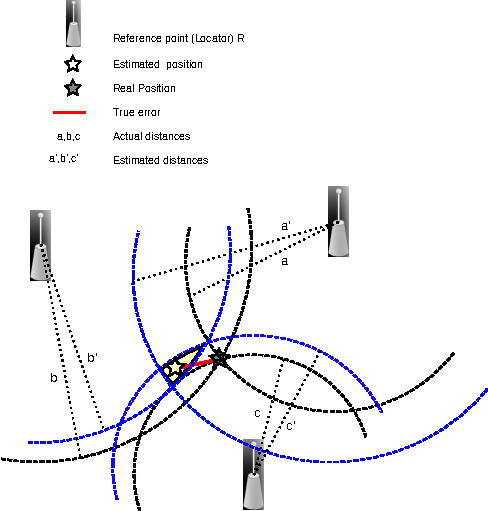
\includegraphics[height=0.4\textheight]{img/uwb_toa.pdf}
          \caption{TOA}\label{fig:uwv-toa}
        \end{subfigure}
        \hfill
        \begin{subfigure}[b]{0.355\textwidth}
          \centering
          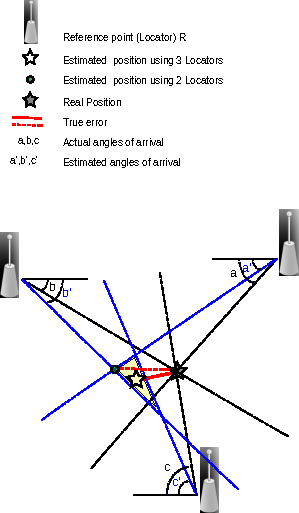
\includegraphics[height=0.4\textheight]{img/uwb_aoa.pdf}
          \caption{AOA}\label{fig:uwv-aoa}
        \end{subfigure}
        
        \caption[Porovnanie princípu metód UWB lokalizácie]{Porovnanie princípu metód UWB lokalizácie~\cite{alarifiUltraWidebandIndoor2016}}\label{fig:uwb}
      \end{figure}

    Technológia \acrshort{uwb} je sprevádzaná aj viacerými nevýhodami a~výzvami. Nakoľko je frekvenčné pásmo zdieľané aj s~inými bezdrôtovými technológiami (napr.\ \acrshort{wimax}, 3G), môže dochádzať k~rušeniu signálu. V~prípade lokalizácie viacerých objektov môže taktiež dochádzať k~problémom s~prístupom na kanál. Spracovanie impulzov z~tagov si vyžaduje komplexný hardvér a~pre presnú lokalizáciu je potrebná presná časová synchronizácia zariadení. Na korekciu chýb spôsobených nedostatočnou synchronizáciou sa používajú rôzne filtračné a~optimalizačné metódy a~algoritmy, napr.\ metóda najmenších štvorcov, Kalmanove filtre či časticové filtre~\cite{al-okbyUWBBasedRealTimeIndoor2024}.

    \subsection{Systémy na snímanie pohybu}
    Systémy na snímanie pohybu (\acrshort{mocap}) boli vyvinuté na zaznamenávanie pohybu objektov alebo ľudí, pôvodne za účelom analýzy chôdze~\cite{furtadoComparativeAnalysisOptitrack18}. Technológia sa však postupne rozšírila aj do ďalších oblastí vrátane robotiky.

    Najpoužívanejšími prístupmi k~\acrshort{mocap} v~posledných rokoch sú~\cite{furtadoComparativeAnalysisOptitrack18}:
    \begin{enumerate}
      \item \emph{opticko-pasívny}~--~najpraktickejší a~najpoužívanejší spôsob v~súčasnosti; sledovaný objekt je označený retroreflexnými značkami (markermi), ktoré sú zaznamenávané viacerými infračervenými kamerami. Každý marker musí byť zachytený viacerými kamerami, jeho polohu je potom možné určiť trianguláciou s~chybou pod 1 mm;
      \item \emph{opticko-aktívny}~--~sledovaný objekt je označený infračervenými LED diódami, ktoré sú snímané infračervenými kamerami. Princíp určovania polohy je rovnaký ako v~predošlom prípade, hlavná nevýhoda však spočíva v~nutnosti napájania aktívnych markerov;
      \item \emph{video}~--~každá snímka je spracúvaná softvérom na detekciu objektov. Dosahuje menšiu presnosť než riešenia využívajúce markery;
      \item \emph{inerciálny}~--~je nezávislý od kamier, využíva inerčné snímače. Slabou stránkou je krátkodobá presnosť.
    \end{enumerate}
  
    Súčasným lídrom v~oblasti \acrshort{mocap} je opticko-pasívny systém OptiTrack. Predstavuje jedno z~najmodernejších riešení lokalizácie objektov, vyznačujúce sa nízkou latenciou, vysokou presnosťou, relatívne jednoduchým používaním a~schopnosťou zaznamenať všetkých 6 stupňov voľnosti (\acrshort{dof}) ako u~pozemných (\acrshort{agv}), tak u~lietajúcich (\acrshort{uav}) autonómnych vozidiel~\cite{MotionCaptureRobotics}. Často sa využíva na validáciu počítačového videnia či ako referencia pre iné metódy lokalizácie. Praktický je hlavne vo vnútorných laboratórnych podmienkach~\cite{furtadoComparativeAnalysisOptitrack18} (viď obr~\ref{fig:optitrack}). Medzi jeho hlavné nevýhody patrí potreba priamej viditeľnosti medzi kamerami a~značkami, výrazný pokles presnosti mimo optimálnej oblasti, vysoké náklady, inštalačná náročnosť a~tiež nevhodnosť použitia v~exteriéri.

    \begin{figure}[b!]
      \centering
      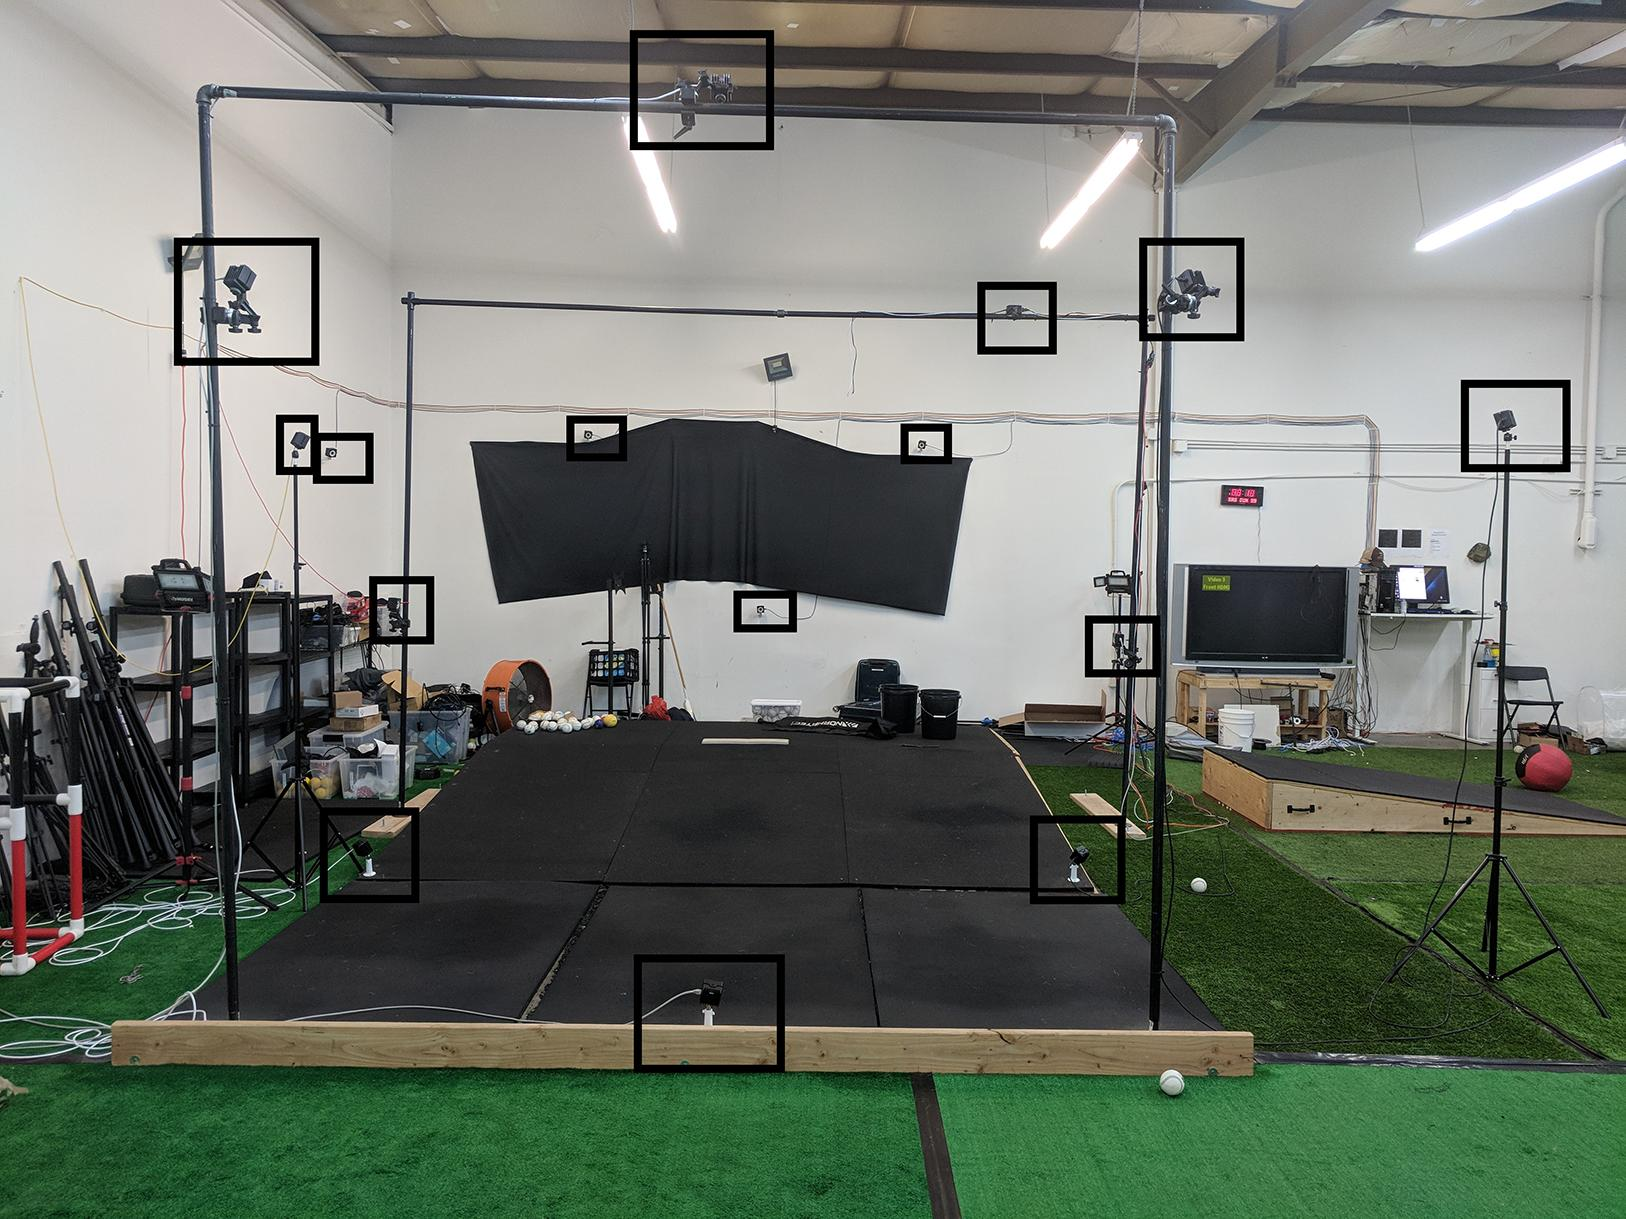
\includegraphics[width=0.85\textwidth]{img/optitrack.jpg}
      \caption[Infraštruktúra pre sledovanie pohybu pomocou systému OptiTrack]{Infraštruktúra pre sledovanie pohybu pomocou systému OptiTrack~\cite{boddyExploringWearableSensors2019}}\label{fig:optitrack}
    \end{figure}

